% MS-Thesis
\documentclass[11pt]{mvlthesis}
\usepackage[dvipdfmx]{graphicx}
\usepackage{verbatim,amssymb,amsmath,subfig,tabularx,ragged2e,booktabs}
\usepackage{float}
\usepackage{adjustbox}
\usepackage{rotating}
\usepackage{cite}
\usepackage{url}
\usepackage[breaklinks = true]{hyperref}
\hypersetup{
  colorlinks = true,
  linkcolor  = red
}
\usepackage{fancyvrb}
\usepackage[]{mcode}

%%%%%%%%%%%%%%%%%%%% SET UP ALL THE TITLE PAGE VARIABLES %%%%%%%%%%%%%%%%%%%
\title{\scshape \mbox{Title Line 1}\\
\scshape \mbox{Title Line 2}}

\author{Joseph Murphy}
\thesis_or_diss{Thesis}
\degree_type{Master of Science}
\field{Electrical and Computer Engineering}
\degreeyear{December 2022}
\chair{Professor Alexander Wyglinski}
\chairtitle{Major Advisor}
\membertwo{Professor Carlo Pinciroli}
\memberthree{Professor Shamsnaz Bhada}
\memberfour{Professor Bashima Islam}

%%%%%%%%%%%% SPECIFY WHICH PARTS OF THE THESIS YOU WANT PRINTED %%%%%%%%%%%%
\renewcommand{\baselinestretch}{1.5}
\newcommand{\pderiv}[2]{\mbox{$\frac{\displaystyle \partial #1}{\displaystyle \partial #2}$}}


%%%%%%%%%%%%%%%%%% Done with setup, document starts here %%%%%%%%%%%%%%%%%%%
\begin{document}

%%%%%%%%%%%%%%%%%%%%%%%%%%%%% TITLE + ABSTRACT %%%%%%%%%%%%%%%%%%%%%%%%%%%%%
\maketitle
\begin{abstract}

As networks and the Internet become more important for work and entertainment and stuff, research into testing new network technologies and topologies continues to grow. % Better motivation wording
This testing can be expensive and time-consuming to do via hardware and so many simulation tools have been created to allow for initial testing without the need for expensive hardware and time-consuming setup.

This thesis examines one such tool, the Extendable Mobile Ad-hoc Network Emulator (EMANE).
This open-source tool can be used to allow for accurate testing of wireless networks by emulating key characteristics of a wireless communication system.

This thesis outlined three separate use-cases for EMANE, testing rural broadband deployment topologies, developing and testing new networking software and hardware, and integrating with other simulation tools to enhance communication accuracy.


\end{abstract}

%%%%%%%%%%%%%%%%%%% ACKNOWLEDGEMENTS + TABLE OF CONTENTS %%%%%%%%%%%%%%%%%%%
\begin{frontmatter}

\begin{acknowledgements}
\begin{center}
\vspace{0.4in}
Acknowledgements
\end{center}
\end{acknowledgements}

\tableofcontents
\listoffigures
\listoftables

\end{frontmatter}

%%%%%%%%%%%%%%%%%%%%% INCLUDE THE REST OF THE DOCUMENT %%%%%%%%%%%%%%%%%%%%%
\chapter{Introduction}
\label{ch:introduction}
The need for wireless communications and network technology is rapidly growing.
As more and more devices become network-enabled, the need for technology to support this rapid growth in wireless communication systems becomes apparent.
Despite this need for interconnectivity, there is still a large divide in the amount of people with access to broadband services.
A study conducted in early 2021 found that rural broadband deployments are increasing, but rural communities still lag behind suburban and urban communities in terms of connectivity~\cite{digital_divide}.
Additionally over the last 10 years, the number of U.S. adults that rely on the Internet has grown by 10\%~\cite{broadband_factsheet}.
This heavy reliance on networks and the Internet is expected to continue, with experts estimating in the next 10 years, the number of IoT devices alone will triple from ten billion to thirty billion~\cite{iot_spread}.
The demand for new wireless technologies and systems creates an issue with testing and deployment.
Part of the reason rural communities lag behind is due to the difficulty in rapidly developing, deploying, and testing communication technology.
To attempt to minimize this issue several tools have been created at allows for testing networks, besides hardware deployments that seek to lower the difficulty of testing.\par

Many software and combination software-hardware platforms exist for testing networks.
Tools like ns-3, MATLAB, and GNURadio all provide different platforms that testing can be conducted.
MATLAB is a good tool for doing signal processing, but simulating the behavior of networks is not a feasible use for it.
ns-3 provides great support for network protocols, but abstracts are made at the physical layer that may call into question the validity of the tool in some use cases.\par

Despite several tools existing to test networks, the issue of cost, accessibility, and accuracy are still rampant.
Many of the tools that have highly accurate models of the entire OSI model, from the physical layer through the transport layer, are very expensive and not attainable.
NetSim and OPNET (now part of the Riverbed platform), provide enterprise grade modeling, but can cost hundreds of dollars to use.
GNURadio allows for interactions with wireless communication hardware and software defined radios, but the hardware component is still an expensive cost looking to be avoided.
Another issue with several of the existing tools is there complexity to set up.
Many tools require extensive programming knowledge to be able to achieve the desired result, or do not provide an easy mechanism with which to analyze results.\par

This thesis proposes several solutions to contribute to the field of network and communications testing:
\begin{itemize}
    \item The Extendable Mobile Ad-hoc Network Emulator (EMANE) is proposed as a valuable testing tool that addresses issues with other similar networking simulation tools. An overview of installing and using the tool is provided.
    \item An initial program designed to maximize bandwidth usage in a constrained wireless network is developed. This is used as an example of how EMANE can be used as a network software development environment.
    \item Basic integration between EMANE and the robot swarm simulator ARGoS is created. EMANE is shown to be capable of extending and enhancing other tools to provide accurate communication emulation when required.
\end{itemize}\par

The remainder of this thesis is organized as follows:
Chapter 2 presents an overview of the network emulator EMANE and the motivation behind the selection of this tool. An overview of the how to use EMANE and its subsystems is presented.
Three different use-cases for the EMANE tool are considered to evaluate the effectiveness of the tool.
Chapter 3 proposes the first use case for testing with EMANE, testing rural broadband deployments. Two similar network topologies are proposed and tested with the help of EMANE.
Chapter 4 explores a second use case for utilizing EMANE, development of networking technologies and systems. In this case a program for more intelligent allocated limited bandwidth is developed.
Chapter 5 finally details a third use case for EMANE, integrating with other simulation tools to provide more accurate communication models.
The paper is concluded with a summary of work completed and recommendations for future work in Chapter 6.

\chapter{Overview on Network Emulation}
\label{chapter2}
Before utilizing the EMANE tool and presenting several situations in which we can use the tool, we must first understand why EMANE was selected and why network emulation is used over simulation or hardware testbeds in this thesis.
After justifying the choices behind selecting EMANE, an in-depth tutorial on the tool's installation, configuration, and operation is presented.
Finally, a brief overview of mobile ad-hoc network (MANET) routing is presented.
These protocols are essential to understand as they are commonly used in EMANE to create routes between nodes.\par

\section{Testing Communication Networks} % General information on network emulation and simulation and hardware testbeds
There are typically three ways new network architectures, technologies, and protocols are developed and tested. These are network simulation, network emulation, and hardware testbeds~\cite{simulation_emulation}.
As expected, each of the three methods has pros and cons as shown in Table~\ref{simtable}.\par
    % Network Hardware
        % Expensive
        % Time consuming to deploy
        % Errors can be sporadic
Hardware testbeds are the most accurate since they encompass the devices expected to be used in the network once development and testing are done.
However, hardware is expensive to purchase, time-consuming to deploy, and often difficult to troubleshoot if errors do not consistently appear~\cite{nsclick}.
These factors make hardware testing not accessible to users that have a low budget.\par
    % Network Simulation
        % Mimic the behavior of a network
        % Uses mathematical models
        % Can run faster than real time
Network simulation is one solution to testing that solves many issues with testing on hardware.
Several free and open-source network simulators such as ns-3~\cite{ns3} or OMNeT++~\cite{omnet++} are commonly used and provide a solution to the high hardware costs.
Similar to most network simulators, these simulators operate on the concept that the behavior of a network and its components can be modeled via statistical and mathematical models.
Creating models for network behavior allows simulators to run faster than real-time since the models do not need to wait for events to happen.
However, the caveat is that simulation models must be highly accurate when developed, or results from the simulation will not match expected hardware behavior.
Researchers creating new simulation models must ensure the models are validated against the expected hardware behavior to confirm the accuracy of the models before they can be used in testing~\cite{omnet_manager}.
Simulation also has the benefit of being highly repeatable since the behavior of the network can be more tightly controlled, and any random processes can be set up to repeat previous random outputs~\cite{simulation_emulation}.\par
    % Network Emulation
        % Operates on real network data
        % Allows integration with hardware
        % Potentially more overhead
Network emulation exists somewhere between testing on hardware and testing inside a simulation.
These emulators are still software that gets used to mirror the behavior of a testbed, such as simulators.
However, emulators operate on actual network data instead of modeling the behavior of a network.
Since emulation testbeds operate on actual network traffic, they also can interface with hardware.
This hardware-in-the-loop functionality allows hardware testing without the need to build an entire hardware network.
This characteristic of operating on real network traffic also has the downside of introducing more computational overhead.
The system emulating the network needs to manage all the test traffic as well as the effects and permutations that are imparted on the traffic.\par

% Table summarizing differences between three methods
\begin{table}[!ht]
	\caption{Pros and Cons of Different Types of Network Testing}
	\begin{adjustbox}{width=\textwidth, center=\textwidth}
		\begin{tabular}{|l|l|l|}
			\hline
			Testbed Type & Pros                                                                                                                                                                       & Cons                                                                                                                                                                  \\
			\toprule
			Hardware     & \begin{tabular}{@{\labelitemi\hspace{\dimexpr\labelsep+0.5\tabcolsep}}l@{}}Highly accurate\\Does not require modification of networking software\end{tabular}                                 & \begin{tabular}{@{\labelitemi\hspace{\dimexpr\labelsep+0.5\tabcolsep}}l@{}}Expensive to build\\Time consuming to deploy and configure\\Errors can be sporadic\end{tabular}               \\
			\hline
			Simulation   & \begin{tabular}{@{\labelitemi\hspace{\dimexpr\labelsep+0.5\tabcolsep}}l@{}}Free tools available\\Can run faster than real-time\\Easy to reconfigure and modify\end{tabular}                   & \begin{tabular}{@{\labelitemi\hspace{\dimexpr\labelsep+0.5\tabcolsep}}l@{}}Models must be designed to be highly accurate\\Software must be translated to a simulation model\end{tabular} \\
			\hline
			Emulation    & \begin{tabular}{@{\labelitemi\hspace{\dimexpr\labelsep+0.5\tabcolsep}}l@{}}Free tools available\\Can run native implementations of network software\\Can interface with hardware\end{tabular} & \begin{tabular}{@{\labelitemi\hspace{\dimexpr\labelsep+0.5\tabcolsep}}l@{}}Must run in real-time\\Requires higher computational overhead\end{tabular}                                    \\
			\hline
		\end{tabular}
	\end{adjustbox}
	\label{simtable}
\end{table}

\section{Evaluation of Network Testing Tools} % Why EMANE was selected over other tools
During the initial research for this thesis, several network simulation and emulation tools were considered for use in this thesis.
These programs all provide functionality that would achieve the goals of performing inexpensive and less time-consuming network testing but were eventually decided against in favor of EMANE.
This section will highlight a few of these tools and explain the reasoning behind why they were not selected before finishing by introducing EMANE and explaining the driving reasons for its selection.\par

% ns-2 and ns-3
One of the most common tools, ns-3, is a discrete event-based network simulation tool commonly used to simulate TCP/IP networks~\cite{ns3}.
It is the successor to the ns-2 tool~\cite{ns2}, with the two significant differences being how simulation scripts are written and executed in the simulator.
In ns-3, the core simulator and experiment scripts are written in C++. ns-3 also provides Python bindings so smaller scripts can be written using Python instead.
This makes ns-3 much simpler than ns-2, which required the use of Tcl scripts to create experiments~\cite{ns2_ns3}.
The migration from ns-2's programming method to ns-3's makes the tool easier to use.
However, it still requires a significant amount of programming knowledge to understand how to utilize the library of models provided.
Being one of the most commonly used tools, ns-3's library of simulation modules has been extensively validated, but these modules typically focus on the network layer and above.
ns-3 can be used as an emulator; however, the motivation for the emulation mode in ns-3 was primarily driven by the ability to use ns-3 with hardware~\cite{ns3_orbit}.
Since we want to avoid wireless hardware equipment, this option for ns-3 is not valuable for the research present in this paper.
The wide-scale use and extensive support of ns-3 made the tool a promising candidate, but it was decided against due to the abstractions made at the physical layer.\par

% OMNeT++
OMNeT++ is another discrete event simulator written in C++, similar to ns-3.
However, OMNeT++ it is not explicitly designed as a communications network simulator~\cite{omnet++}.
Despite not being designed as a communications network simulator, the ability to create plugins for the tool has led to many researchers creating models of communication networks that can be used.
The issue with this collection of plugins is that many users have found them to be highly incompatible with each other.
This is likely due to the isolated nature many of the modules were developed under~\cite{tool_survey}.
One of the advantages of OMNeT++ is that it supports a graphical user interface that allows for more accessible building of and interaction with network testbeds.
Figure~\ref{omnet_gui} shows an example of this GUI, which is based on the Eclipse IDE.
Since OMNeT++ is not designed for communications networks specifically and many plugins are incompatible, it was decided not to be used.

\begin{figure}[!ht]
    \centering
    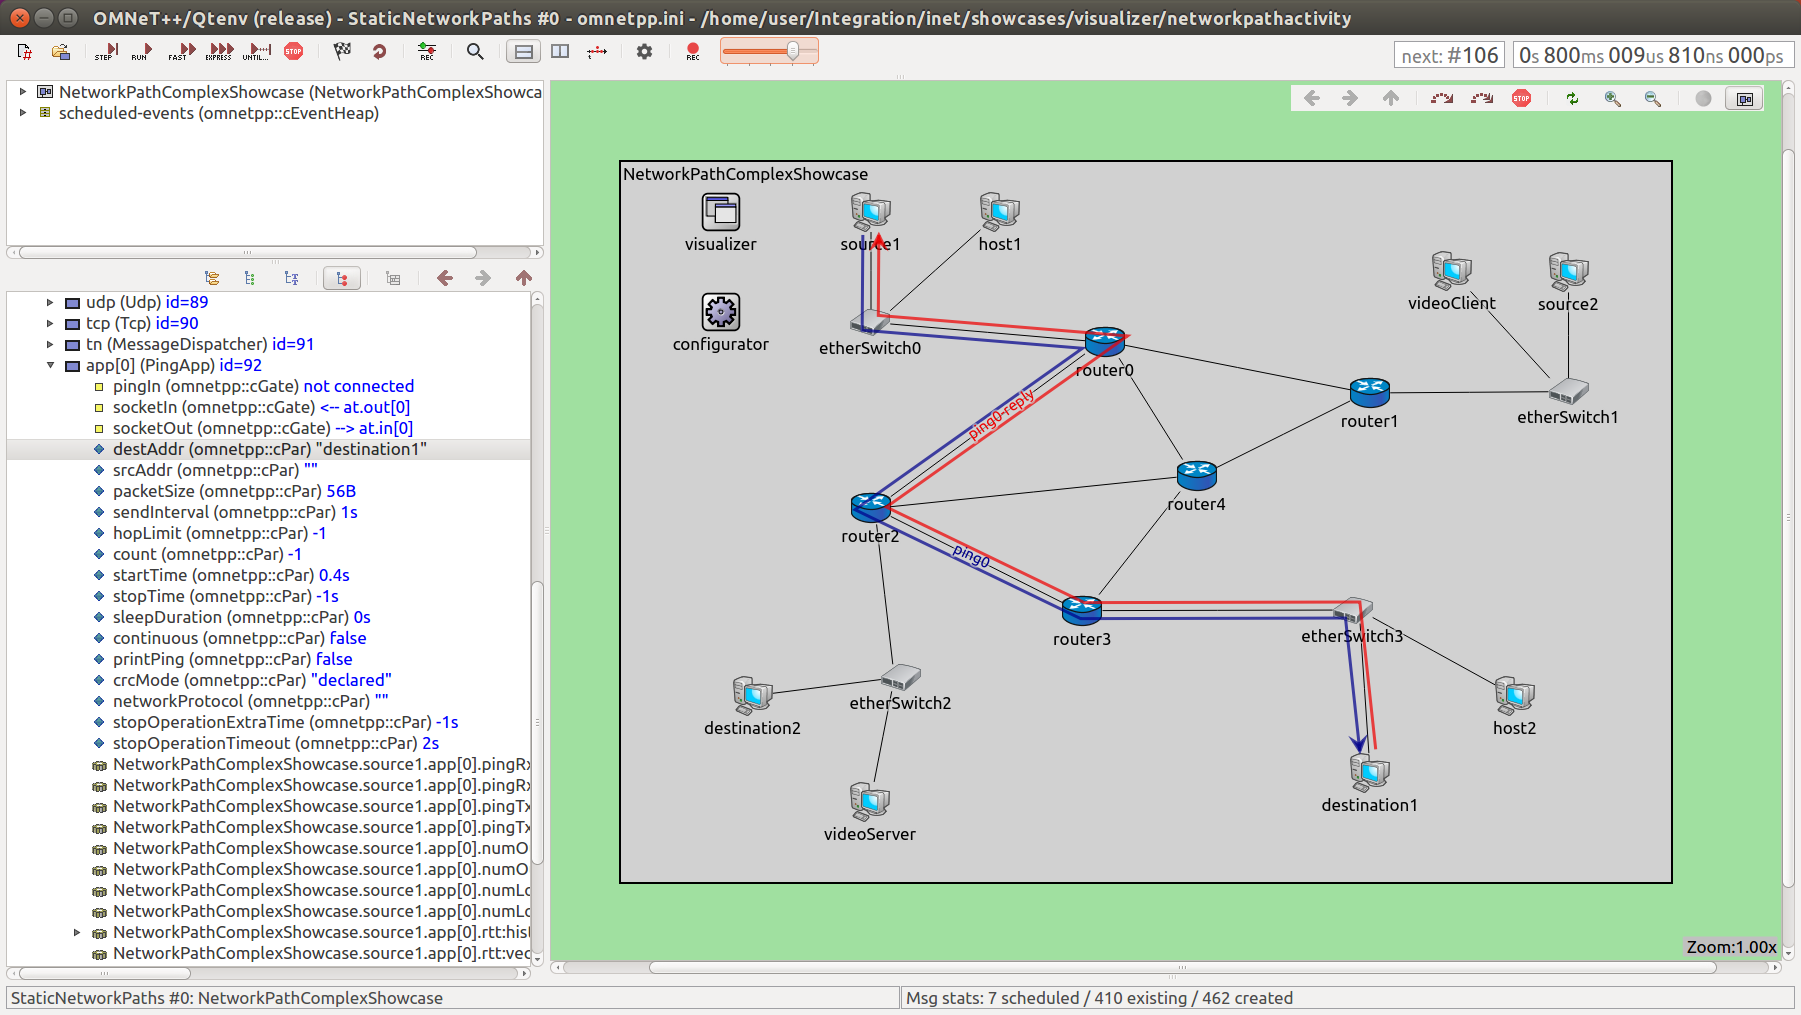
\includegraphics[width=\textwidth,keepaspectratio]{Images/Chpt2/omnet_gui.png}
    \caption{An example of the OMNeT++ Simulator GUI (from~\cite{omnet++}).}
    \label{omnet_gui}
\end{figure}

% CORE
The Common Open Research Emulator (CORE) is an emulation tool focused on the emulation of layers three (network layer) and above in the OSI stack \cite{core}.
Of all the tools presented so far, CORE is one of the easiest to use.
Similar to OMNeT++, CORE provides the user with a GUI that takes the form of a blank canvas where users can drag and drop preconfigured nodes, such as routers and servers, into a network implementation.
Figure~\ref{core_gui} is a basic example of how a typical CORE session appears.
CORE also allows users to create virtual nodes via a Python framework, which is helpful for more complex scenarios.
Without any modification, CORE emulates the network layer and above perfectly, as each virtual node is running the actual, unmodified software that would be running on hardware \cite{emane_core}.
Where CORE runs into issues is when wireless channels are introduced.
By default, CORE operates on the concept that if nodes are close enough to communicate, they have a perfect connection, and if they are far enough apart by a certain distance, they can not communicate.
This simplification is not acceptable for most testing requiring accurate wireless communication modeling. To solve this issue, EMANE was integrated into CORE so that all physical and data link layer emulation happened through EMANE instead~\cite{emane_core}.
Figure~\ref{core_emane} shows the configuration menu for EMANE within CORE.
With this pairing, CORE and EMANE become a very valuable tool.
However, in this thesis CORE is not used independently or alongside EMANE.
The main reasoning is that most protocols being used at the network layer or higher are not present in CORE, and computational complexity can be saved by running them in EMANE directly, without CORE.\par

\begin{figure}[!ht]
    \centering
    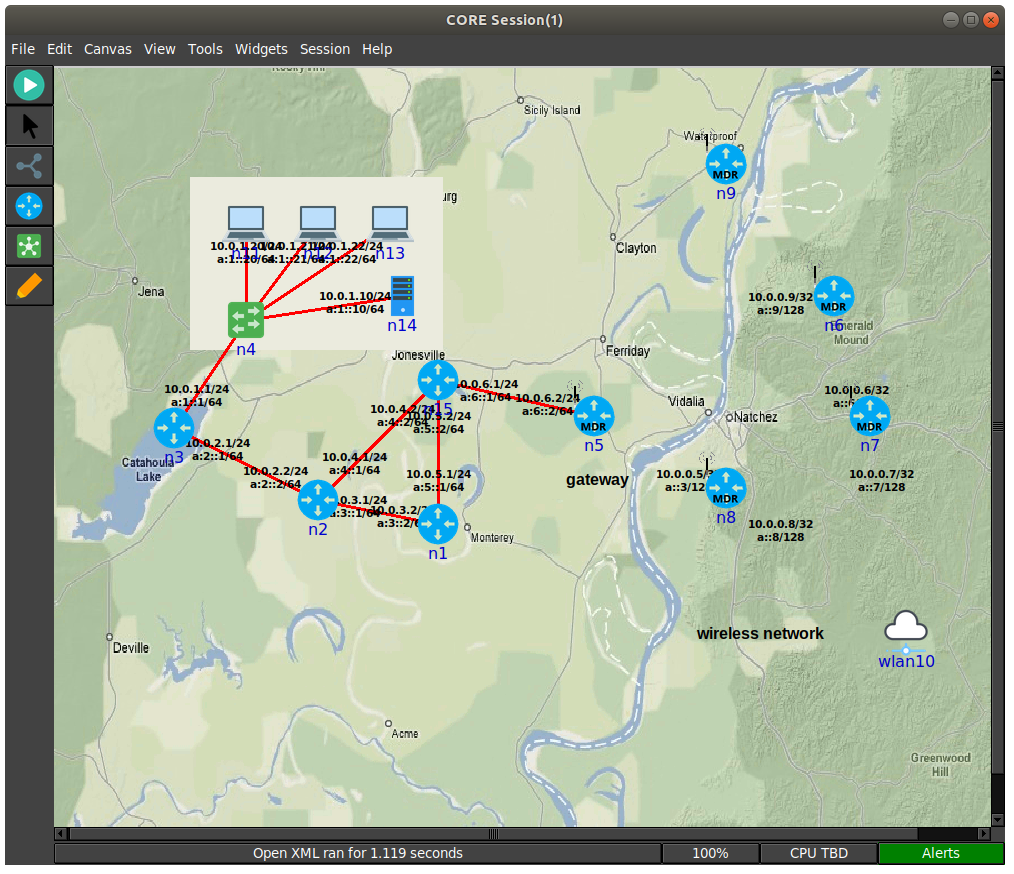
\includegraphics[width=0.7\textwidth,keepaspectratio]{Images/Chpt2/core_gui.png}
    \caption{An example of the CORE Emulator GUI (from~\cite{core}).}
    \label{core_gui}
\end{figure}

\begin{figure}[!ht]
    \centering
    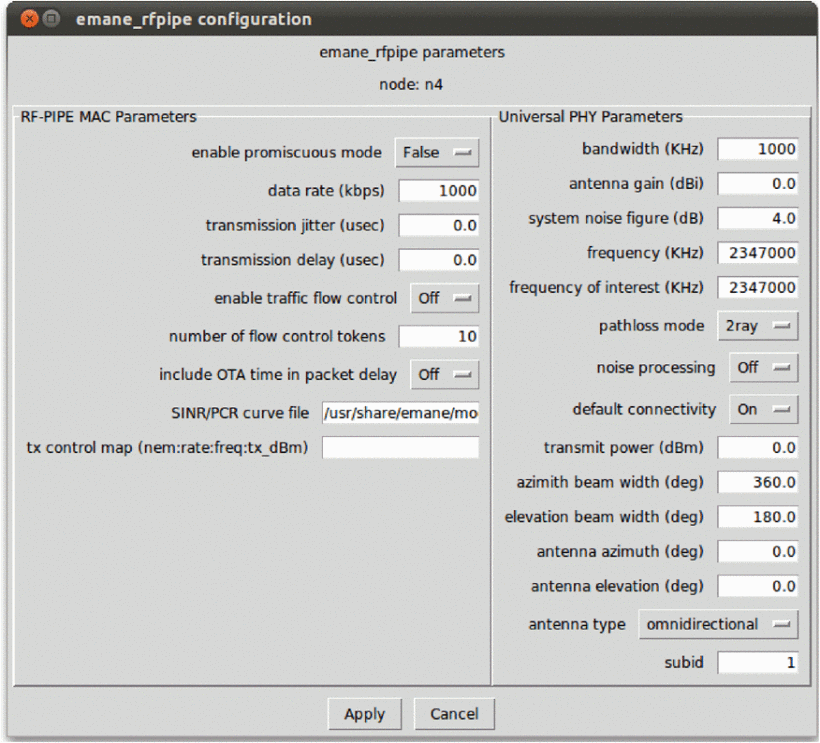
\includegraphics[width=0.7\textwidth,keepaspectratio]{Images/Chpt2/core_emane.png}
    \caption{The configuration menu for EMANE, within CORE (from~\cite{emane_core}).}
    \label{core_emane}
\end{figure}

% EMANE
EMANE is a network emulation tool originally developed by the Naval Research Lab and currently maintained by AdjacentLink LLC~\cite{emane_nrl}.
The tool is a discrete event-driven emulator programmed in C++ and Python, and is configured by the user primarily through XML files and Bash scripts.
The software was developed with the intention of creating a platform that could emulate the physical and data link layers of the OSI network model with high accuracy, therefore avoiding many of the abstractions made by other tools.
EMANE consists of several subsystems and components required to create a fully functional testbed, and this complexity can lead to an initial steep learning curve with the tool.
However, given that the tool is open-source, the online community around EMANE is rather small and most of the discussion and troubleshooting surrounding the tool is only found on EMANE's GitHub issues page, not helping solve the initial complexity issue.
Despite all this, once the user forms a solid understanding of the tools and systems within the software, it can be used to effectively and quickly create wireless networks.
EMANE's ability to be configured through XML files makes deployment of networks very rapid, and because the included models are pluggable, these configuration files can be reused in other networks using the same wireless technology.
For these reasons and the reasons highlighted previously regarding other testing tools, EMANE was selected as the tool of choice for this thesis.
The next section is dedicated to understanding how to install the tool, and how all the pieces work together.\par

Table~\ref{tooltable} highlights the main advantages and disadvantages of each of these tools.

\begin{table}[!ht]
	\caption{Overview of Advantages and Disadvantages of Different Networking Testing Tools}
	\begin{adjustbox}{width=\textwidth, center=\textwidth}
        \begin{tabular}{|l|c|c|} 
        \hline
        \multicolumn{1}{|c|}{Tool} & Advantages & Disadvantages \\ 
        \toprule
        ns-3 & \begin{tabular}[c]{@{}c@{}}Open-source\\Extensive protocol library\\Widely used and validated\end{tabular} & \begin{tabular}[c]{@{}c@{}}Abstracts the PHY and MAC layers\\Limited control of individual nodes\\Simple wireless propagation models\end{tabular} \\ 
        \hline
        OMNeT++ & \begin{tabular}[c]{@{}c@{}}GUI-based\\Large library of models\end{tabular} & \begin{tabular}[c]{@{}c@{}}Not purpose built for network simulation\\Provided models are often not compatible\end{tabular} \\ 
        \hline
        CORE & \begin{tabular}[c]{@{}c@{}}Open-source\\GUI-based\\Simple models do not require programming knowledge\end{tabular} & \begin{tabular}[c]{@{}c@{}}Only emulates the network layer and above\\Limited network protocols available by default\end{tabular} \\ 
        \hline
        EMANE & \begin{tabular}[c]{@{}c@{}}Open-source\\Purpose built to emulate PHY and MAC layer\\Can use any implementation of network software\end{tabular} & \begin{tabular}[c]{@{}c@{}}Small online community\\Initial steep learning curve\\Requires extensive computing resources for large-scale networks\end{tabular} \\
        \hline
        \end{tabular}
	\end{adjustbox}
	\label{tooltable}
\end{table}

\section{Using EMANE}
Having selected EMANE for use in this thesis, we must now understand how to install, configure, and operate the tool.
This section will begin by detailing the installation of EMANE.
The primary two methods of installation are using the bundle of pre-built binaries provided by AdjacentLink or building all the required programs from source.
Compiling the software from source is typically only necessary when making extensions to the tool, such as adding custom modules.
Since only the default included modules are used in this thesis, the precompiled bundle is sufficient for our purposes.
The installation instructions for EMANE can be found in~\cite{emane_tutorial}, but it should be noted that these instructions are sometimes out of date.
The full EMANE GitHub repository~\cite{emane_git} may also provide guidance that is more up to date.
EMANE version 1.3.3 was the primary version of the tool used in this work, and this version supports the Rocky 8, Fedora 37, and Ubuntu 20.04 Linux distributions.\par
    % Basic installation instructions
        % Download binary packages
        % Install pre-complied bundle
        % Verify programs are installed
        % Optionally: Install extra software
These instructions assume a fresh installation of Ubuntu 20.04.4 is being used and that the system is up-to-date with the latest software.
If a different supported distribution of Linux is used, the steps will be similar, however the exact commands will differ. Refer to~\cite{emane_tutorial,emane_git} for further details.
See Appendix~\ref{appendixa} for a list of the specific commands used to complete the entire installation process.
\begin{enumerate}
    \item The first step is downloading the precompiled binaries. As seen in Figure~\ref{wget_emane}, the \textit{wget} utility is used to download the compressed file, but any method for retrieving this file can be used. This compressed file should be extracted before the next step.
    \item To install the downloaded binaries, the \textit{dpkg} application is used. Errors will be reported upon installation, as not all the dependencies are installed. This will be fixed after the initial installation via \textit{apt}. Figure~\ref{install_emane} shows the initial installation finishing with errors, and the command used to fix these errors.
    \item Lastly, we can verify that EMANE was installed correctly by having the program output its version. Figure~\ref{check_emane} shows that EMANE version 1.3.3 was successfully installed.
    \item Once installation of EMANE has been verified, additional support software (such as testing tools and routing protocols) can be installed to use with EMANE. Appendix~\ref{appendixa} shows some examples of installing certain tools.
\end{enumerate}

\begin{figure}[!ht]
    \centering
    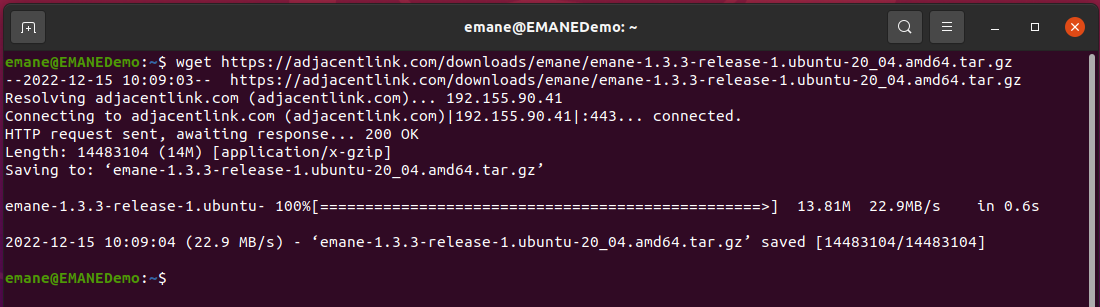
\includegraphics[width=\textwidth,keepaspectratio]{Images/Chpt2/wgetEMANE.png}
    \caption{Downloading the precompiled EMANE binaries using the \textit{wget} command.}
    \label{wget_emane}
\end{figure}

\begin{figure}[!ht]
    \centering
    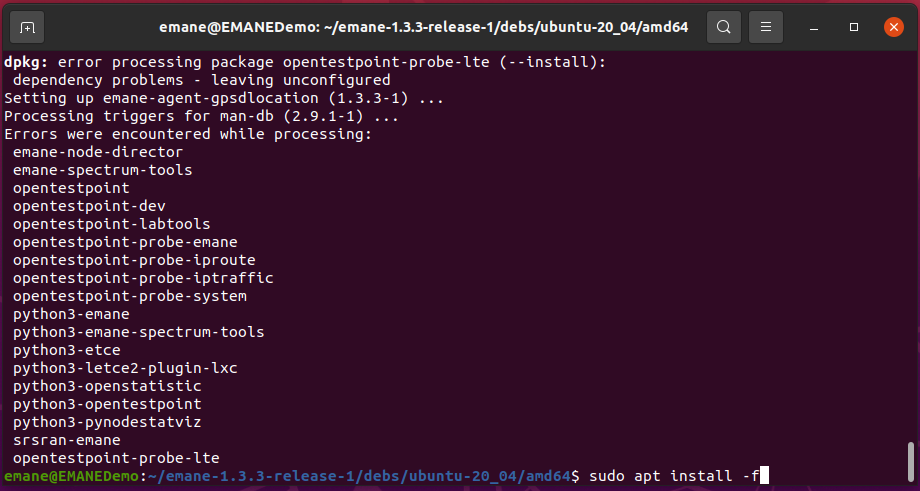
\includegraphics[width=\textwidth,keepaspectratio]{Images/Chpt2/dpkgEMANE.png}
    \caption{Installing the EMANE program \textit{dpkg} command.}
    \label{install_emane}
\end{figure}

\begin{figure}[!ht]
    \centering
    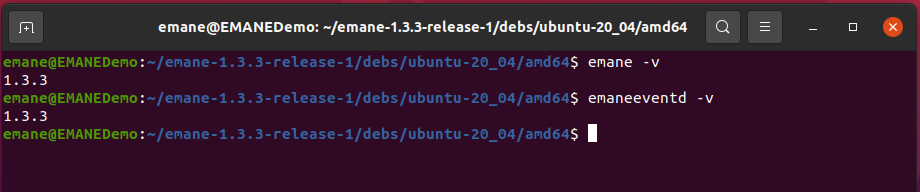
\includegraphics[width=\textwidth,keepaspectratio]{Images/Chpt2/versionEMANE.png}
    \caption{Verifying EMANE installed correctly by displaying the version number.}
    \label{check_emane}
\end{figure}

    % Basic architecture overview
    % NEMs
        % Each NEM should exist on its own platform server inside its own LXC
            % EMANE recommends not putting multiple NEMs on one platform server for performance reasons
            % Each platform server (running instance of EMANE) needs to have network stack isolation (accomplished via LXCs, but other methods exist)
        % Each NEM has 3 layers, PHY layer, Radio layer, and transport layer
        % Each NEM also interfaces with the event engine to ensure proper configuration and processing
Now that EMANE is installed, it is important to understand the major systems that work together to enable network emulation.
The main structure in EMANE that everything operates around is known as the Network Emulation Module (NEM).
Each NEM can be thought of as a single network node, similar to a singular radio.
As each NEM is an independent network node, every NEM created requires network stack isolation within the kernel of the host system.
All the traffic flowing through the emulation testbed consists of real IP packets and are therefore treated in the same way as regular network traffic by the kernel.
If the network stacks were not isolated, packets would not route through the emulator and would instead just be switched between processes in the kernel, bypassing all wireless channel effects.\par
There are several methods than can be used to create network stack isolation.
Full virtual machines could be used, but these are very computationally inefficient and would not allow the emulated testbed to maintain a large number of nodes.
Additionally, nodes in EMANE do not need the full isolation provided by virtual machines, and it is even beneficial if the file system could be shared.
To solve this problem, containers are used as the primary method of isolation.
\cite{core_containers} examines several types of virtualization that can be used for isolation nodes in CORE, but the same concepts apply to EMANE.
Between FreeBSD jails, Linux OpenVZ containers, and Linux namespaces containers, the namespaces containers are found to be the most efficient.
For most examples of EMANE and all the testbeds created in this thesis, Linux Containers (LXCs) are used.
These are lightweight containers that are built on top of Linux namespaces and allow for the sharing of files and other resources, while keeping processes and the network stack isolated.\par

Figure~\ref{emane_diagram} shows how a typical EMANE emulation node appears, with one of these structures existing per LXC.
In this diagram, the NEM is visible, with all of its surrounding subsystems and connections.
The blue boxes within the NEM are the emulation models that are responsible for imparting wireless channel effects on packets moving upstream and downstream through the emulator.
The green boxes represent the transport boundary. This is the edge of the emulation node where packets leave the emulator and return to normal application space.
The orange box represents the event service that is responsible for changing the state and settings of the emulator during runtime in order to create effects in the network.
These three systems are the major subsystems that make up EMANE and allow it to create highly dynamic networks, used to test a variety of situations and will be examined in depth in the next three subsections.

\begin{figure}[!ht]
    \centering
    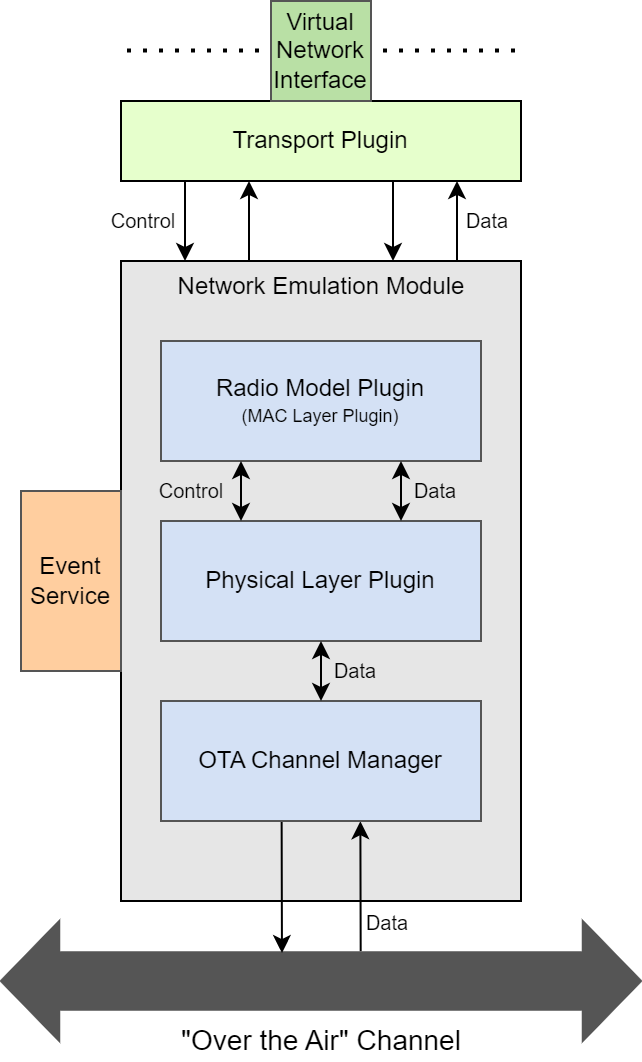
\includegraphics[width=0.5\textwidth,keepaspectratio]{Images/Chpt2/emane_diagram.png}
    \caption{An overview of an individual EMANE emulated network node.}
    \label{emane_diagram}
\end{figure}

\subsection{Emulation Model Processing}
    % Emulation Model Processing
The emulation model processing is the system primarily responsible for modifying packets traveling through the NEM to mimic the behavior of a wireless signal.
This system in EMANE consists of two main parts, the Physical Layer Plugin and the Radio Model Plugin, both of which can be seen in blue in Figure~\ref{emane_diagram}.
As the names of the plugins imply, the Physical Layer plugin is responsible for imparting the effects of the physical layer, and the Radio model plugin is responsible for the MAC Layer.
The Over the Air (OTA) Channel Manager is primarily responsible for pulling packets addressed to the NEM off of the shared bus, and putting packets ready to be transmitted onto the shared channel.
This shared OTA channel simply takes the form of a virtual interface bridge that all NEMs are attached to, creating a bus topology.
The NEMs use a multicast scheme to listen for packets as other control channels also use this interface bridge to communicate.
It is the main backbone of the emulation that connects all the individual network nodes, both for control messages, but also data payloads.\par
    % Shared PHY model
        % Pathloss, fading, noise, pulling packets of OTA channel, power calculations
As previously mentioned, the shared PHY plugin is responsible for the effects of the physical layer.
It is possible to create a custom Physical Layer model, but is usually not necessary and only one PHY model is included in EMANE by default.
This model is responsible for attributes such as path loss and signal propagation, fading, noise modeling, and the antenna profile.\par
The first parameter to be set is the propagation model.
This model is responsible for calculating the expected path loss between two nodes, and has three options.
The first two options are \textit{freespace} and \textit{2ray}.
These use location data contained within the node and the freespace or 2-ray flat earth model to calculate the path loss of a channel.
The third option is called \textit{precomputed} and is used when the path loss is to be calculated external to the emulator.
This is useful if a more complex model is to be used, or a different tool is being used to model signal propagation.\par
The second configuration step is related to the power characteristics of the node and its virtual antenna.
Transmit power can be set, and serves the same purpose it would on a hardware radio.
The antenna gains can be set as a static value, or a more complex profile that contains a list of antenna pattern entries.
The following is an example of the contents of an antenna profile file from the CORE/EMANE documentation~\cite{core}:
\begin{center}
\begin{minipage}{\textwidth}
    \begin{minted}[fontsize=\small, breaklines]{xml}
    <!-- 30degree sector antenna pattern with main beam at +6dB and gain decreasing by 3dB every 5 degrees in elevation or bearing.-->
    <antennaprofile>
      <antennapattern>
        <elevation min='-90' max='-16'>
          <bearing min='0' max='359'>
            <gain value='-200'/>
          </bearing>
        </elevation>
        <elevation min='-15' max='-11'>
          <bearing min='0' max='5'>
            <gain value='0'/>
          </bearing>
    \end{minted}
\end{minipage}
\end{center}\par
The final piece of the PHY model that must be understood is noise modeling.
EMANE models noise by taking the transmission power of any NEM actively transmitting, and adding it to the noise floor of any receiving node if that receiver's set frequency is within the bandwidth of the interfering signal.
This results in all interfering signals being treated as white noise~\cite{emane_phy}.
EMANE provides parameters to set if the noise mode is for all signals within the correct frequency, just signals that are out-of-band, or turning off noise processing completely.
Once all of these factors are set, EMANE can then use the following two equations to determine if a packet can actually be received:
\[ rxPower = txPower + txAntennaGain + rxAntennaGain - pathloss \]
\[ rxSensitivity = -174 + noiseFigure + 10log(bandwidth) \]
If the received power (\textit{rxPower}) is greater than the receiver's sensitivity (\textit{rxSensitivity}), the packet is received.
Figure~\ref{emane_phy} shows how a general Physical Layer Plugin configuration file appears.\par

\begin{figure}[!ht]
    \centering
    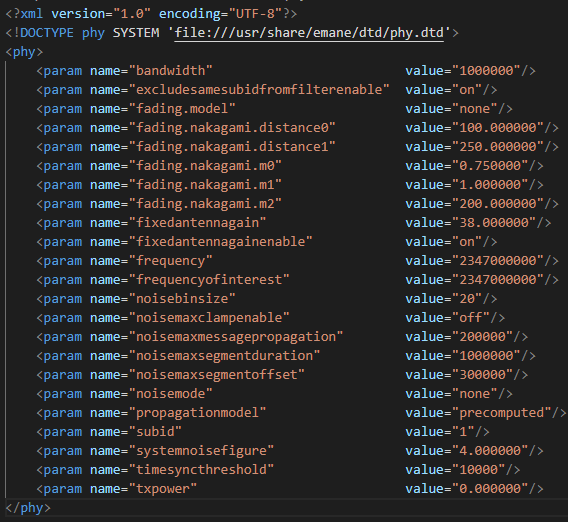
\includegraphics[width=0.8\textwidth,keepaspectratio]{Images/Chpt2/emane_phy.png}
    \caption{A generic configuration file for an EMANE PHY Plugin}
    \label{emane_phy}
\end{figure}

    % Radio model
        % Data bandwidth, delay, more advance medium access control schemes, SINR packet drop probabilities
The second piece of the emulation model processing layer of EMANE is the Radio Model plugins.
Unlike the PHY plugin which is shared for all NEMs, the Radio plugin is different depending on the type of waveform emulation desired.
EMANE ships with four Radio plugins:
\begin{itemize}
    \item rfPipe - A generic wireless channel that does not do channel access functions
    \item IEEE802.11abg - A model specifically for 2.4GHz Wi-Fi waveforms
    \item TDMA - A generic time division multiple access scheme
    \item Bypass - A model specifically for testing that passes traffic along to the next layer unchanged
\end{itemize}
Other plugins can be created by extending the emulator, and a plugin designed for LTE and 5G is currently under development in collaboration with the srsRAN project~\cite{srsran,srsran-emane}.\par
These four plugins all operate differently, but for the purposes of this thesis only the rfPipe model will be used.
The goal of rfPipe is to create a simple model that handles data rate, delay, jitter, and probability of packet loss due to signal to interference and noise ratio (SINR).
The data rate, delay, and jitter are all simple parameters that get set and are implemented by holding packets at the radio model layer long enough to achieve the set values.
The Packet Completion Rate (PCR) utilizes the signal, interference, and noise power levels calculated by the Physical Layer model to find the SINR value, and compares that to a lookup table.
The portion of the table and corresponding curves, as seen in Figure~\ref{emane_pcr}, are used to come up with a probability value that is used to decided if the packet should be lost or otherwise corrupted due to noise.

\begin{figure}[!ht]
    \centering
    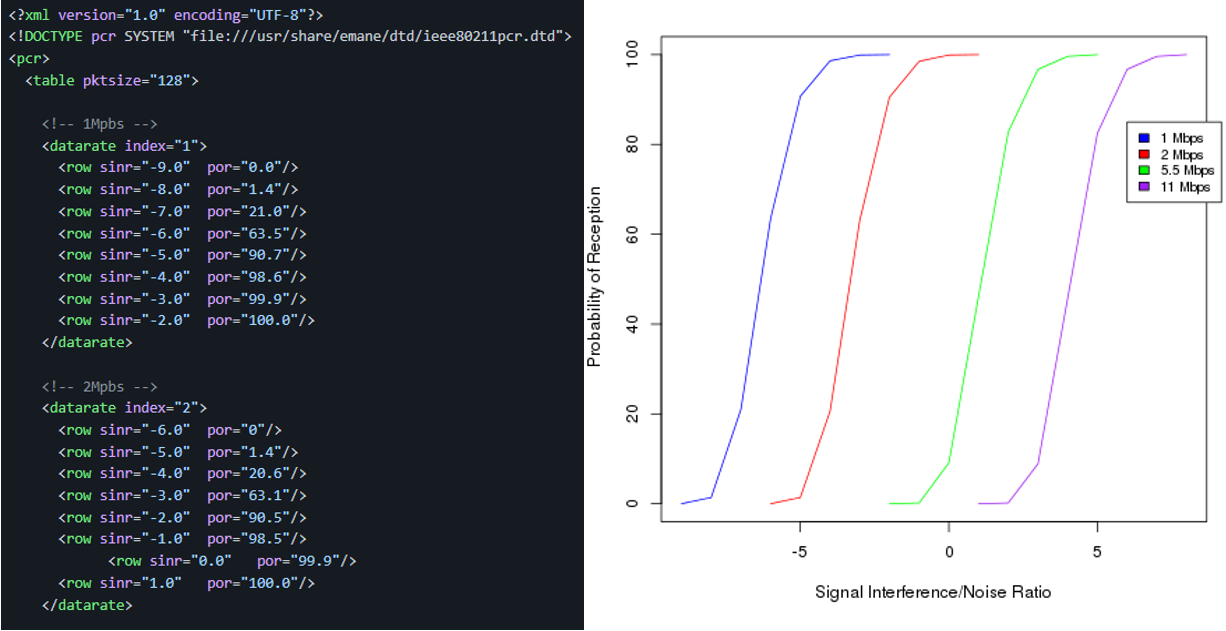
\includegraphics[width=\textwidth,keepaspectratio]{Images/Chpt2/emane_pcr.png}
    \caption{The packet complete rate (PCR) table and corresponding curve.}
    \label{emane_pcr}
\end{figure}

One of the essential pieces of the emulation processing system is ensuring the models used are accurate to hardware, to ensure results from the emulator are accurate.
While several studies use the rfPipe model \cite{rfPipe1, rfPipe2, rfPipe3}, very little literature could be found validating the models included within EMANE.
The rfPipe model is generic enough that there are no modulation schemes or other access functions that need to be validated, but the implementation of the behavior must still be checked.
Similarly, the calculations performed at the Physical Layer are fairly simple, but must also be validated.
A validation similar to the one found for the time-divison multiple access (TDMA) model \cite{emane_tdma}, should be performed for all models presently in EMANE, as well as for any custom models created.
For the purposes of this thesis, EMANE is being used to test parameters such as throughput and latency which can be easily compared to hardware equivalent testbeds.
Chapter~\ref{chapter3} will examine this to make comparisons between the two, however, if EMANE is to be used in more advanced testbeds with highly complex models, validation is essential.

\subsection{Transport Boundary Processing}
    % Transport Boundary Processing
The second system required to operate EMANE is the transport boundary.
The transport boundary is represented in Figure~\ref{emane_diagram} by the green boxes, and is responsible for handing packets entering and exiting the emulator.
Since EMANE is capable on operating on actual TCP/IP packets, one of the main roles of the transport boundary is to translate TCP/IP packets entering the emulator into something EMANE can operate on, and translate EMANE's packet back into TCP/IP packets.
There are two types of transports that can be used with EMANE: raw transports and virtual transports.\par
    % Raw transport
        % Use physical network device as edge of emulation
        % Allows for "black-box" style testing
        % Can be used to interface physical networking hardware with EMANE
Raw transports are used for enabling the hardware in the loop functionality of EMANE.
When a raw transport plugin is initialized, it is connected to a hardware network interface present on the emulation host machine.
This breaks the convention of having EMANE nodes exist within LXCs, but if only one EMANE node is present on the host the node can run external to a virtualized environment.
If multiple nodes exist, a pair of virtual network interfaces can be created and bridged to the hardware interface to create a tunnel from inside the LXC to the hardware interface on the host.
This method is used in Chapters 3 and 4 and will be outlined in more detail there.
Figure~\ref{emane_raw_transport} shows an example of the layout of the network interface on the host and the EMANE instance.

\begin{figure}[!ht]
    \centering
    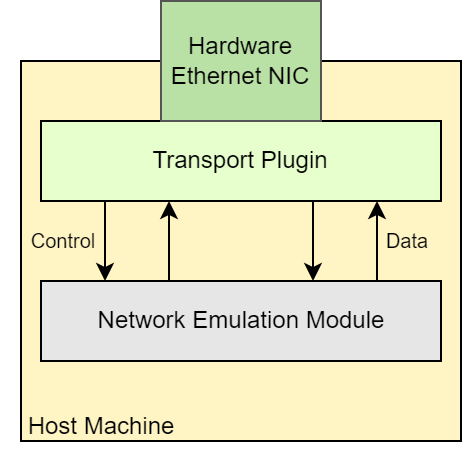
\includegraphics[width=0.4\textwidth,keepaspectratio]{Images/Chpt2/RawTransport.png}
    \caption{An example EMANE topology using the raw transport plugin.}
    \label{emane_raw_transport}
\end{figure}

    % Virtual transport
        % Uses virtual kernel interfaces as edge of emulation
        % Internal transports
            % For NEMS on the same platform server, packets are not even sent through kernel devices, just shared with each other in memory
        % External transports
            % NEMs on different platforms servers must share data through the kernel (since they will have network stack isolation)
The second type of transport are virtual transport plugins.
These are more the commonly used plugins that carry data from the emulator instance to application space via a virtual network interface.
When EMANE is started in an LXC using a virtual transport, the LXC is created with a pair of virtual interfaces.
One of the interfaces is internal to the LXC and is used as the endpoint for EMANE, the other is external to the LXC and is bridged together with all the other nodes to allow traffic to pass.
Figure~\ref{emane_virtual_transport} shows an example layout of the virtual network interfaces bridged together between EMANE instances, internal on the host machine.

\begin{figure}[!ht]
    \centering
    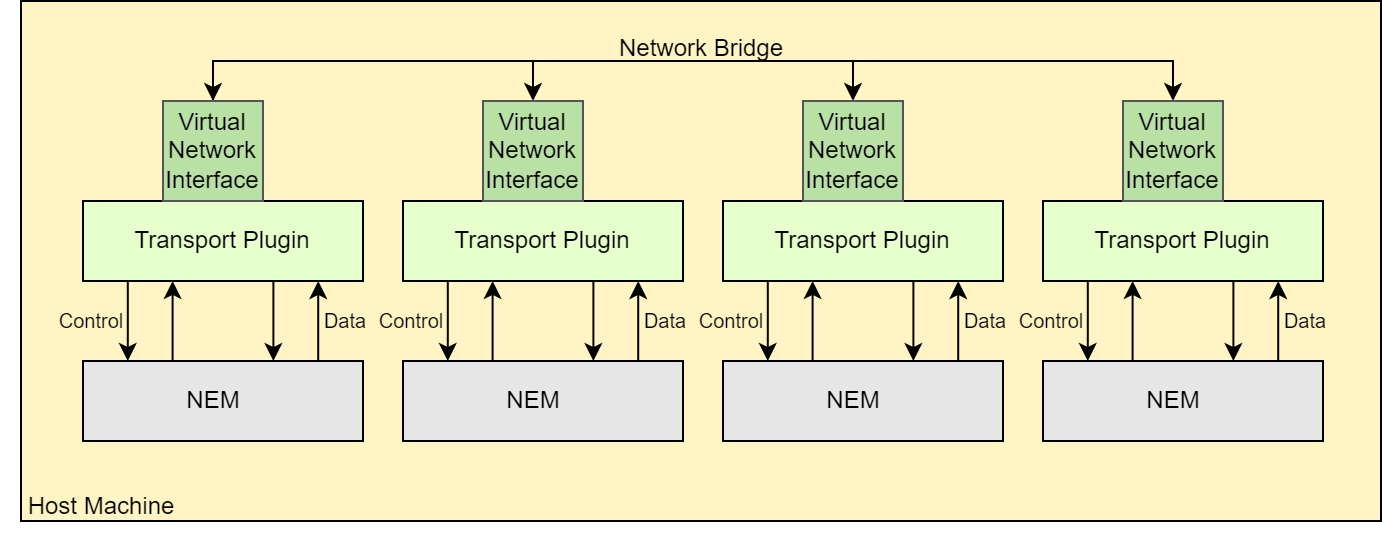
\includegraphics[width=\textwidth,keepaspectratio]{Images/Chpt2/VirtualTransport.png}
    \caption{An example EMANE topology using the virtual transport plugin.}
    \label{emane_virtual_transport}
\end{figure}

\subsection{Event Processing}
    % Event Processing
        % Event channel vs. OTA channel
            % Scripted before runtime
                % EEL file(s)
            % Sent during runtime
                % Python modules
Event processing is the system in EMANE that allows parameters of the simulator to change during runtime.
There are five main event types.
The first type, ``pathloss'', is used when the propagation model is set to \textit{precomputed} and allows an external tool to make path loss calculations.
The second type, ``location'', is used to move nodes around and primarily influences path loss values that are calculated internally to the tool when using \textit{freespace} or \textit{2ray} settings.
The location event can take latitude, longitude, altitude, pitch, yaw, roll, and velocity data for a node.
The third event type is the ``antenna profile'' event.
Similar to the antenna profile setting in the Physical Layer plugin, this event can be used to feed antenna data to a node, and change that data during runtime.
The fourth event is used to change the fading model being used.
This event is fairly simple and is used to toggle whether a node uses the Nakagami fading model or no fading model.
The final event is called ``Comm Effect'', and is used to change generic communication parameters of a node, such as the latency, jitter, or probability of packet loss and duplication.\par
    % Scripted before runtime
        % EEL file(s)
    % Sent during runtime
            % Python modules
There are two primary methods by which events get generated for distribution to nodes.
The first is using an EEL file.
This file is a specific EMANE file that is taken in at the start of emulation and contains ``sentences'' that outline event parameters and what time during the simulation they should begin.
Figure~\ref{emane_event} shows an example of an EEL file and the sentences contained within.
The first value is the time the event is scheduled to fire, in this case all of these events fire at the start of emulation.
The second value is the ID of the NEM the event is destined for, and this is followed by the event name and any corresponding parameters for that event type.
The other main method for generating events is through Python bindings that allow direct subscription to the event channel for publishing of events.
Events are passed to NEMs via the event channel, but all this channel is, is a different multicast service that the NEMs subscribe to on the same virtual network interface bridge that the over the air channel lives on.
By putting both of these channels on the same bridge, the complexity of managing several network devices per NEM is lessened.

\begin{figure}[!ht]
    \centering
    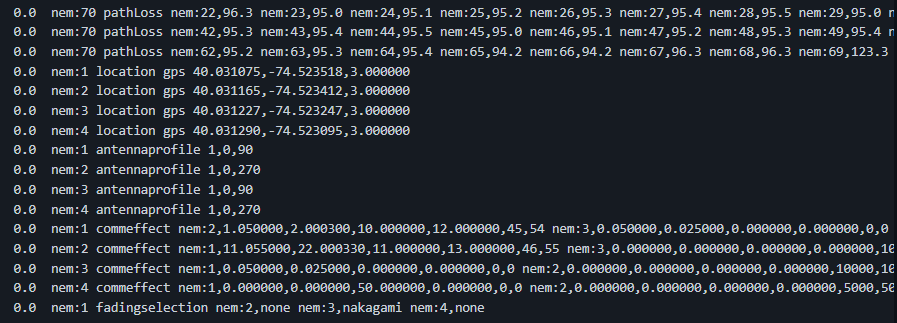
\includegraphics[width=\textwidth,keepaspectratio]{Images/Chpt2/emane_event.png}
    \caption{An example of an EEL file provided to the EMANE event service.}
    \label{emane_event}
\end{figure}

\section{Routing in Mobile Mesh Networks}
    % What is important in routing in a ad-hoc mobile network rather than a traditional network
    % What routing algorithms exist in literature
        % Reactive vs. Proactive
EMANE was designed originally to work with mobile ad-hoc networks (MANETs).
While emulating other network types is possible, MANET routing protocols work well with EMANE's architecture and are often used.
This special classification of network is characterized by its dynamic topology that often rapidly changes due to the mobility of network nodes and the tendency for the wireless links to intermittently connect and disconnect~\cite{manet_storm}.
This lack of a fixed topology means that any node that exists in the network must be able to communicate without help from centralized infrastructure or a gateway and therefore must be able to independently make routing decisions. 
Since the topology of a MANET is a mesh, the primary method for traffic traveling through the network is through relaying.
Each node in the mesh acts as a router and upon receiving network traffic, must determine if the traffic is destined for itself, or a different node in the network.
In the second case, the relaying node will use its knowledge of the routing table and network topology to determine which neighbor node the packets must be forwarded to~\cite{manet_survey}.
These types of routing protocols can be separated into two categories, proactive protocols and reactive protocols~\cite{manet_survey}.

\subsection{Proactive Mesh Routing}
        % Requires more overhead
        % Can (keep can, not will) react more quickly to topology changes
        % Periodically send out "discovery" packets to sense link quality/delivery topology info/etc.
The first category of MANET routing protocol is the proactive protocol.
Proactive protocols are similar to traditional routing protocols in the sense that they create and maintain a routing table.
By maintaining a routing table, any transmission that needs to be sent can be done so immediately since the most efficient route is known.
This allows proactive protocols to operate with less latency than reactive MANET routing protocols as they do not need to wait for route discovery at the time of transmission~\cite{manet_performance}.
The caveat to this is that these protocols require much higher control traffic as they must perform periodic link sensing to ensure the routing tables are up-to-date.
In a network where bandwidth is constrained, it is essential to understand this limitation at the time of design as MANETs are often already bandwidth restricted and adding another high usage system could create instability in the network.\par
        % Examples:
            % OLSR
                % Floods network with topology info
            % BATMAN-adv
                % Layer two routing, node only aware of neighbors
                % Depends on neighbors to ensure data is passed along
There are two routing protocols that the maintainers of EMANE often use in examples and tutorials for the tool.
These are the Open Link State Routing (OLSR) protocol~\cite{rfc_olsr} and the Better Approach to Mobile Ad-hoc Networking (B.A.T.M.A.N.) protocol~\cite{batman}. 
These routing protocols are both proactive MANET routing protocols and are two of the more common purpose built proactive protocols found in MANETs.
They both operate on the similar principle of link sensing via a discovery packet (called HELLO packets in OLSR and OGM packets in B.A.T.M.A.N.), but differ in how the best routes are calculated.\par
        % BATMAN general performs better than OLSR in most conditions [cite paper]
When deciding between these two protocols it is found that B.A.T.M.A.N. typically will outperform OLSR~\cite{olsrd_batman}.
This can be attributed to the manner in which OLSR performs link sensing.
When evaluating two paths, the path with the least number of relays is considered the best path in OLSR~\cite{rfc_olsr}.
This concept is feasible in high speed wired networks where queuing and relaying of data is often the slowest portion of a packets journey, but in wireless networks where the quality of the medium can drastically vary, this does not work as well.
B.A.T.M.A.N. attempts to solve this issue by using identifying the link that first delivers an OGM packet from a new node.
That identified link is then flagged as the best way to send a packet to the node indicated in the new OGM.
Since the link with the lowest latency and highest throughput is expected to deliver packets the fastest, it can be assumed it is the best link~\cite{batman}.
Since B.A.T.M.A.N. nodes only measure which neighbor has a route to a given destination, and does not share the topology of the entire network graph, the protocol also produces less control traffic, which contributes to it performing better.
Figure~\ref{batman_topology} shows what topology information nodes might have in a network running B.A.T.M.A.N.
Nodes B and C maintain a list that indicates which nodes in the graph are accessible through each neighbor. In this example, node B does not know the layout of connections between nodes C, D, E, and F.
It is only aware that C has the best route to all of those destinations, and relies on C's routing table to relay the packets the rest of the way.
This has the benefit of making topological changes that occur on the opposite side of the mesh transparent to nodes not immediately effected, reducing the amount of traffic that needs to occur when the mesh changes.

\begin{figure}[!ht]
    \centering
    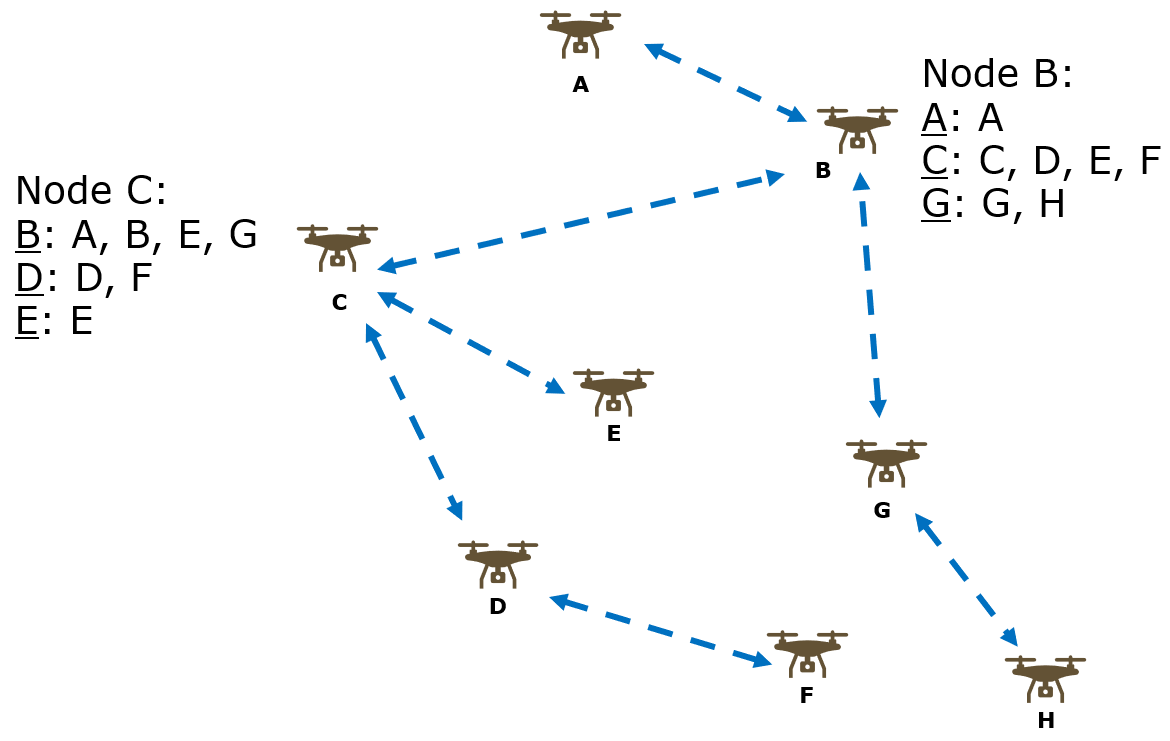
\includegraphics[width=\textwidth,keepaspectratio]{Images/Chpt2/BATMAN_topology.png}
    \caption{An overview of an individual EMANE emulated network node.}
    \label{batman_topology}
\end{figure}

\subsection{Reactive Routing}
    % Does not require maintenance and therefore generates less traffic
    % Topology updates are only discovered when a previously discovered route fails
The other primary category of MANET routing protocol are reactive protocols, also sometimes referred to as ``on-demand'' protocols~\cite{manet_survey}.
These protocols are referred to as on-demand protocols because routes to a destination are only found when the transmitting node requires them.
This has the benefit of greatly reducing control traffic present in the network since topology and link state information is not periodically shared, but it does result in higher latency as traffic must wait for a route to be found.
This type of routing protocol could be beneficial in a network that is constrained on bandwidth and will typically only contain traffic that is not time-sensitive.\par
    % Examples:
        % AODV
        % DSR
Two examples of reactive MANET protocols are AODV and DSR~\cite{reactive_routing}.
These protocols generally act by sending out request packets upon needing a route, indicating the destination the traffic is intended for, and waiting for a response.
Nodes that have a route to that destination respond, and once a full route is found the traffic is sent.
The route is then stored and considered a good route for that destination until an attempt at using the route fails.
At that point the discovery process is repeated to find a new route.\par
    % BATMAN tends to have less available bandwidth than AODV, but more reliably delivers packets and detects topology changes faster
Generally, reactive protocols are found to not be as effective in highly mobile MANETs \cite{aodv_batman,reactive_routing}.
B.A.T.M.A.N. is found to have less maximum available bandwidth in some situations when compared to AODV, but will more reliably deliver packets successfully, and often is able to react to changes in the graph faster.
For this reason, proactive protocols such as OLSR and B.A.T.M.A.N. are more commonly used in simple EMANE testbeds, as seen in the tutorial~\cite{emane_tutorial}.\par
All the testbeds in the remainder of this thesis will use the batman-adv implementation of the B.A.T.M.A.N. protocol.
This implementation is built into the Linux kernel and installation instructions for using it can be found in Appendix~\ref{appendixa}.

\section{Chapter Summary}
    % Chapter covered the basics of EMANE so that it may be used to set up and run experiments
    % Mobile ad-hoc routing is important to understand the operation of the robot swarm experiment
This chapter covered necessary background information on the differences between testing networks in hardware, testing networks in simulation, and testing networks in emulation.
Network hardware testbeds are expensive and so simulation or emulation were decided to be used instead.
Several network simulators including ns-3, OMNeT++, CORE, and EMANE were examined, and the emulator EMANE was determined to be the best tool for this thesis thanks to its accurate modeling of the PHY and MAC layers, mechanisms to individually control the software running on each node, and ability to interface with hardware.
Having selected EMANE, installation instructions were detailed, and an overview of the tool and its subsystems was presented.
The chapter then finished by presenting an overview of MANET routing protocols, the type of protocol that will be used in the created EMANE testbeds.    %% Overview on Network Emulation, EMANE, bandwidth scheduling, and mesh routing

\chapter{Hybrid Wireless Rural Broadband Networks}
\label{chapter3}
The first testing scenario EMANE was placed under was emulating two wireless, hybrid network topologies that were designed to more effectively deliver broadband to small rural communities.
Since deploying broadband to rural communities can be expensive through traditional methods, wireless distribution topologies have become a popular way of bringing the Internet to these communities.
As was explained, testing wireless networks in hardware is rather expensive, and finding a location that meets the environmental factors of the target rural communities is challenging.
To solve these issues, initial testing can be conducted in EMANE. This allows an understanding of the interactions between the technologies selected to be formed, and do basic validation that the proposed network can feasibly achieve its goal.

\section{Hardware Testbed Network Topologies}
    % Hardware testbed utilized a mmWave backhaul and Ubiquiti LTU radios for the distribution network
        % mmWave and LTU were abstracted using rfPipe in EMANE
    % Allowed for testing throughput and bandwidth characteristics with multiple hosts connected as well as range using simple pathloss models
Both of the network architectures that will be examined in this chapter were eventually set up in hardware.
While these hardware testbeds were being built, emulated EMANE testbeds were also set up.
Both testbeds can be classified by two distinct wireless technologies, the first stage is a millimeter wave (mmWave) backhaul.
This wireless, high data rate backhaul was intended to replace the traditional wired backhaul, that makes reaching these rural communities so difficult.
The other technology used was Ubiquiti's proprietary LTU protocol~\cite{ltu}.
The LTU leg of the network consisted of the distribution portion of the network and was responsible for bridging the connected houses to the backhaul.
By abstracting both of these technologies into EMANE, testing characteristic behaviors of the network with several hosts was possible.
A pfSense router~\cite{pfsense} was also used in both testbeds to handle all routing requirements.
Thanks to EMANE's hardware in the loop capabilities, the actual pfSense software was used in the experiment emulation testbed.

\subsection{OVERCOME Testbed}
    % Topology
        % (FIGURE\_OVERCOMETopology)
        % Two sets of mmWave backhauls
        % Aggregate at a router in the middle of town
        % Split into 3 radios for distribution to ~30 houses
The first of the two testbeds was located in Turney, Missouri (39°38'09.9``N 94°19'14.3``W), a small community outside of Kansas City that was not currently covered by any of the Internet Service Providers in the area.
The topology of the network can be seen in Figure~\ref{overcome_topology}.
\begin{figure}[!ht]
    \centering
    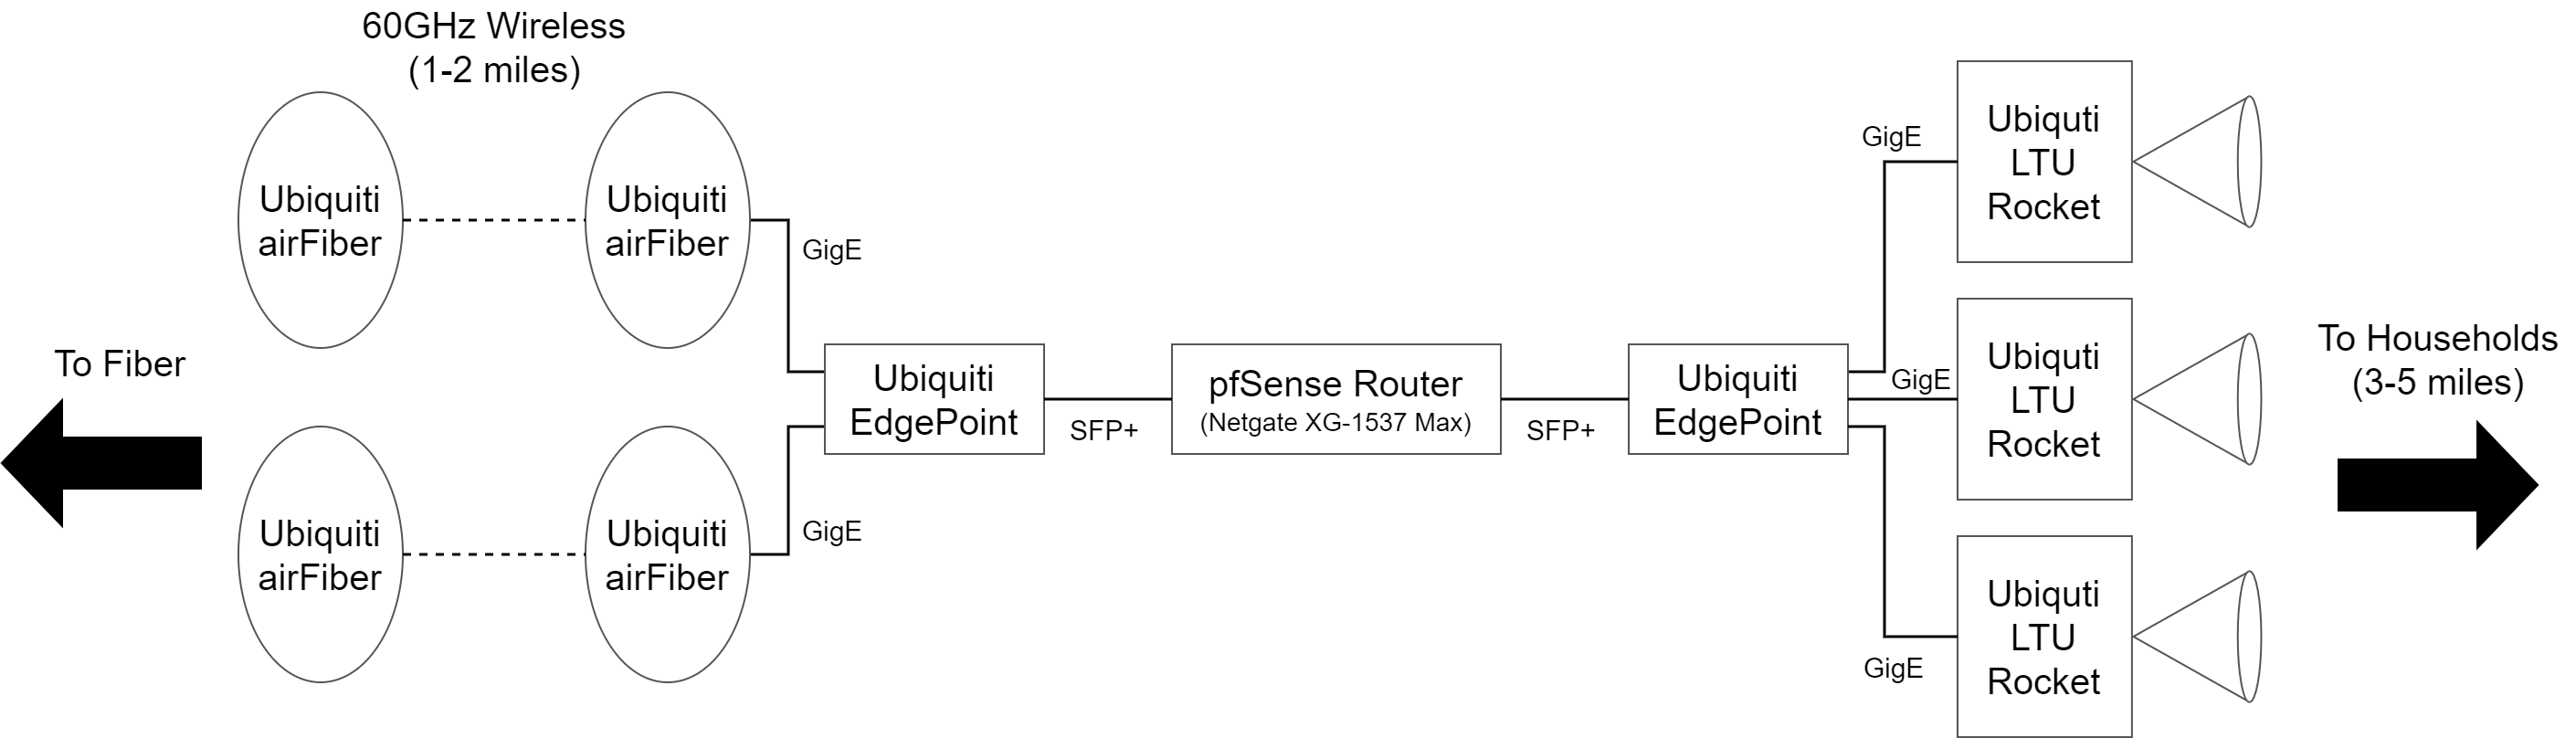
\includegraphics[width=\textwidth,keepaspectratio]{Images/Chpt3/OVERCOME_Topology.png}
    \caption{The network topology of the testbed built as part of Project OVERCOME~\cite{projovercome} in Turney, MO.}
    \label{overcome_topology}
\end{figure}
In order to create this topology in EMANE, we first had to understand the major characteristics of the hardware being mimicked.
    % Technologies used
        % Ubiquiti AirFiber, Ubiquiti Edge Switches, Netgate pfSense Router, Ubiquiti LTU Rockets
The mmWave backhaul consisted of four Ubiquiti airFiber 60LR radios~\cite{airfiber}.
These two pairs of point-to-point radios acted as the backhaul of the network and carried the traffic from the nearest location with fiber, to the center of the community.
Once arriving at the center of Turney, the traffic was passed through a commercial Netgate XG-1537 Max router running pfSense~\cite{netgate_1537}.
This router was primarily responsible for switching traffic off the ISP's network and onto the last leg of the network to the homes.
The final piece of the network was the LTU leg.
The transmitting radios from the center of town to all the homes were three Ubiquiti LTU Rockets~\cite{lturocket}.
These radios connected to an Ubiquiti LTU Pro~\cite{ltupro} at each house, which provided Internet connectivity to the user. 

\subsection{ZoomTel Testbed}
    % Topology
        % (FIGURE\_ZoomTelTopology)
        % Two-hop mmWave backhaul
        % LTE-U distribution network at each hop
        % Distribute to hosts centered around each hop
The second testbed topology was not deployed to an actual location where it would be permanently used, and was instead just tested locally.
The topology of what was tested can be seen in Figure~\ref{ZoomTel_topology}.
\begin{figure}[!ht]
    \centering
    \includegraphics[width=\textwidth,keepaspectratio]{Images/Chpt3/ZoomTel_Topology.png}
    \caption{The network topology of the experimental testbed built as part of the ZoomTel project.}
    \label{ZoomTel_topology}
\end{figure}
The primary idea behind this network topology, and what makes it differ from the OVERCOME topology, is that the segment shown in Figure~\ref{ZoomTel_topology} is intended to be repeated and tiled to create a mesh of backhaul connections.
This would allow the pfSense route at the origin of the mesh to make routing determinations based on the quality of links in the network, and could attempt to solve the issue of the delicate nature of mmWave links, especially with respect to weather systems.
In this thesis only the single segment shown in Figure~\ref{ZoomTel_topology} was implemented for testing, but could easily be expanded in EMANE.\par
    % Technologies used
        % Siklu EtherHaul, Ubiquiti network switches, Ubiquiti LTU Rockets
The technologies used in this testbed are similar to the ones in the previous network, but the equipment that implements primarily the mmWave links is different.
In this network, the fiber is directly connected to a pfSense router instead of the backhaul, this allows the special routing functionality that was described.
The hardware network tested in this topology used a generic Dell OptiPlex desktop as the router.
Since the pfSense software is free to use, a commercial solution does not need to be purchased to use it.
All the mmWave links were created using the Siklu Kilo Series EtherHaul 1200~\cite{etherhaul}, four of which were used.
The LTU link used the same Ubiquiti LTU Rocket as the radio located at the backhaul, but unlike the OVERCOME project, the LTU Lite radios~\cite{ltulite} were used as the customer premises equipment (CPE).


\section{Creating the Networks in EMANE}
    % Creating mmWave and LTU in EMANE
        % Use rfPipe to mimic characteristics of mmWave and LTU
            % Bandwidth, delay, throughput, frequency of interest, distance between radios, antenna RX and TX gains
In order to implement the mmWave and LTU wireless technologies into EMANE, the rfPipe model was selected.
Since the primary concern with the emulation testbed was mimicking the general behavior of the network, it was decided the that rfPipe model would work well enough, and a more complex model was not needed.
Table~\ref{mmwave_params} outlines the key configuration parameters that were used to create the mmWave links.
Table~\ref{ltu_params} outlines the same parameters and their selected values for the LTU waveforms.
Since the LTU radios varied between testbeds and the characteristics of the basestation radio and CPE radios were different from each other, values that would most accurately model the average expected behavior were selected.
This could cause some variation in the results, but it was deemed acceptable for the proposed use case.
Most of these parameters were selected based on the datasheets of both radio platforms and the antennas (integrate or external) that were used.
This is information that would be available prior to purchasing hardware to validate a design.
The freespace path loss model was selected as the effects of multipath were not expected to be a primary concern in the testbeds.\par
\begin{table}[!ht]
\centering
\caption{mmWave Model EMANE Parameters}
\begin{tabular}{lr} 
\hline
\multicolumn{1}{c}{EMANE Parameter} & \multicolumn{1}{c}{Value} \\ 
\hline
Delay & 0.5ms \\
Data Rate & 1Gbps \\
Frequency & 60GHz \\
Channel Width & 500MHz \\
Fixed Antenna Gain & 43dBi \\
Path loss Model & \multicolumn{1}{l}{Freespace} \\
\hline
\end{tabular}
\label{mmwave_params}
\end{table}
\begin{table}[!ht]
\centering
\caption{Ubiquiti LTU Model EMANE Parameters}
\begin{tabular}{lr} 
\hline
\multicolumn{1}{c}{EMANE Parameter} & \multicolumn{1}{c}{Value} \\ 
\hline
Delay & 2.5ms \\
Data Rate & 200Mbps \\
Frequency & 5.8GHz \\
Channel Width & 20MHz \\
Fixed Antenna Gain & 19.5dBi \\
Path loss Model & \multicolumn{1}{l}{Freespace} \\
\hline
\end{tabular}
\label{ltu_params}
\end{table}
\begin{figure}[!ht]
    \centering
    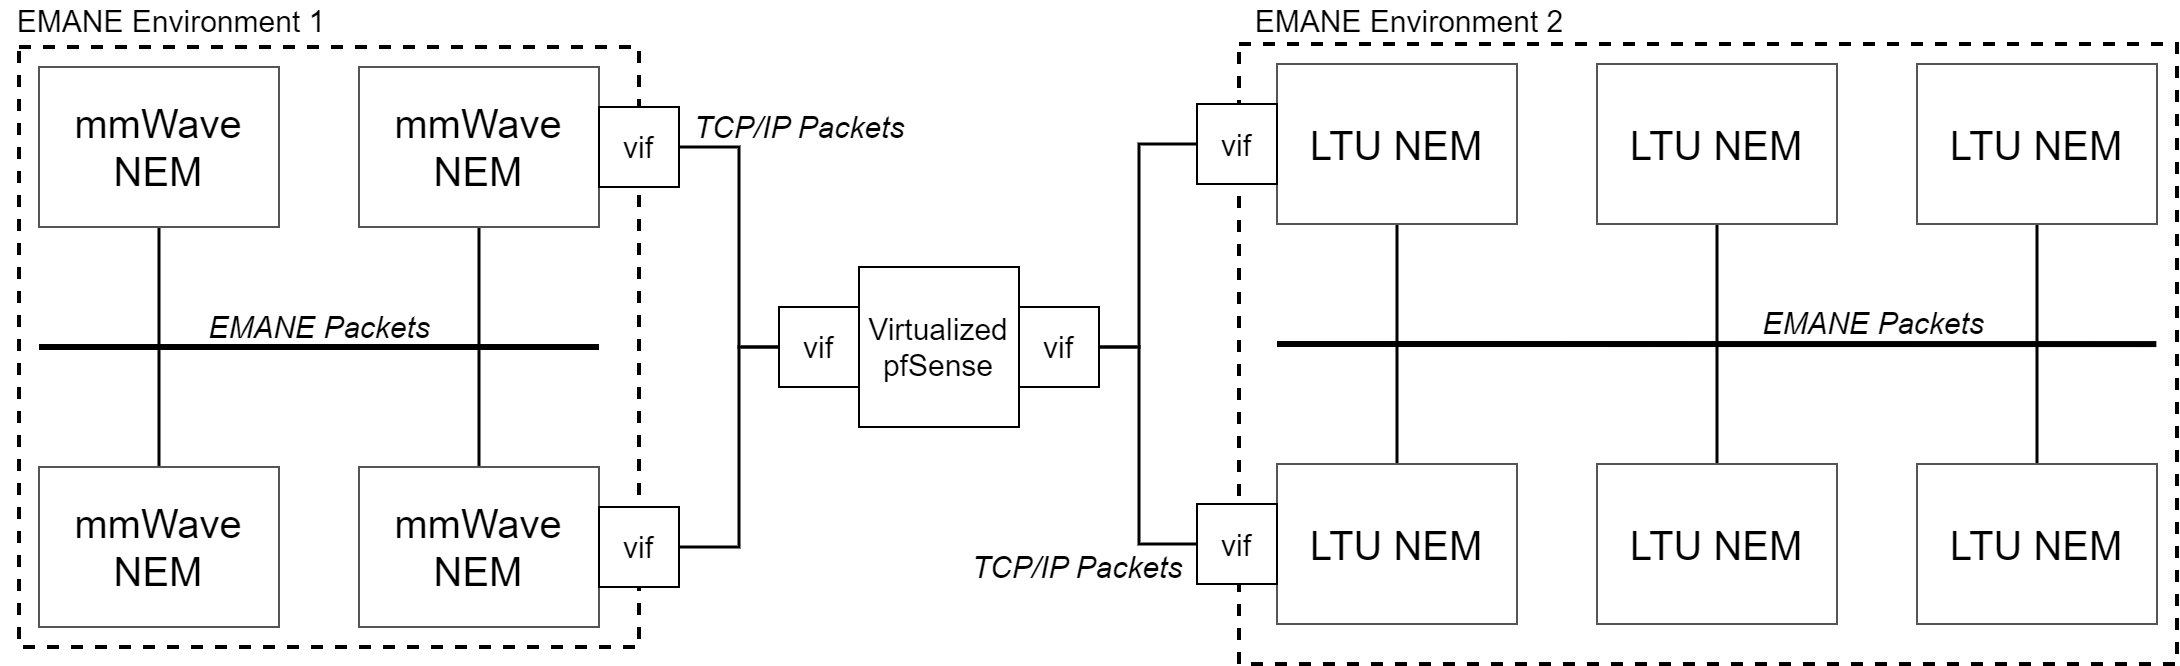
\includegraphics[width=\textwidth,keepaspectratio]{Images/Chpt3/EMANE_OVERCOME.png}
    \caption{The emulation testbed topology corresponding to the OVERCOME project.}
    \label{overcome_emane}
\end{figure}
\begin{figure}[!ht]
    \centering
    \includegraphics[width=\textwidth,keepaspectratio]{Images/Chpt3/EMANE_ZoomTel.png}
    \caption{The emulation testbed topology corresponding to the ZoomTel project.}
    \label{ZoomTel_emane}
\end{figure}
With the radio plugins configured in the NEMs, two EMANE environments were created for the OVERCOME testbed, and three EMANE environments were created for the ZoomTel testbed.
These emulation topologies can be seen in Figure~\ref{overcome_emane} and Figure~\ref{ZoomTel_emane}, respectively.
It is important to note that the two individual mmWave links in the ZoomTel topology are separate EMANE instances.
These could have been put in the same environment as was the case with the OVERCOME testbed.
However, it was elected to make them entirely separate to allow for more control over the events that were used to effect the operational environment.
If a weather system and its effects on the channel were to be modeled, being able to only impart those effects on a single mmWave link is a very useful ability to have, especially if the testbed was developed further to implement the poor link quality avoidance routing system previously described.\par
    % Interfacing with a real pfSense router in EMANE
        % Use EMANE transport plugins to delivery and receive real TCP/IP packets from a virtualized router
        % Performance implications of using a virtualized router vs. the real hardware router?
            % (No, there was such limited traffic that the hardware router was never pushed beyond a few percent usage, and the virtual router never bottlenecked)
In both testbeds, a pfSense router is virtualized and inserted into the emulation loop.
This was initially a difficult process as understanding exactly how the transports needed to be configured to properly pass the TCP/IP traffic to and from the router to emulator was not clear in the documentation.
Several portions of the example configurations use a transport plugin scheme that is later recommended to not be used, causing substantial confusion.
Eventually a tutorial~\cite{letce2_git} and a forum post~\cite{issues_git} were found that detailed exactly how to connect a virtual machine to a NEM container.
The process primarily relies on creating an additional pair of virtual network interfaces that connect the LXC to the host machine, and having VirtualBox~\cite{virtualbox} bridge this interface.
Since this new interface is not a part of EMANE directly, and therefore not a member of any routing schemes, manual routes needed to be configured so the LXC would properly forward the packets to and from EMANE.
This is an example of the code that was used to add these manual routes in the ZoomTel testbed:
\begin{minted}[fontsize=\small, breaklines]{Bash}
#!/bin/bash -
ip route add 10.150.2.0/24 via 10.100.1.2
ip route add 10.100.2.0/24 via 10.100.1.2
ip route add 10.150.3.0/24 via 10.100.1.2
ip route add 10.200.3.0/24 via 10.100.1.2
\end{minted}
This script would run on startup of the initial mmWave LXC node and add routes to the second mmWave emulation network, the LTU network, and the external TCP/IP networks bridging the EMANE instances.\par
One of the important factors taken into consideration when virtualizing pfSense, was if the virtualization of the router software would have performance impacts on the network.
The expectation was that there would not be any major impacts since pfSense is a very lightweight program and is often virtualized in production environments.
For reference, the pfSense router running in production in the OVERCOME project connecting 30 households to the Internet was never recorded at more than a few percent CPU usage.
Similarly, the virtual pfSense router never reached above 5\% CPU usage and the router never indicated it was dropping packets due to computational overload.

\section{Hardware Results versus Emulation Results}
Having built the emulation testbeds, it was time to use them for testing.
Since the hardware testbeds were already in the process of being built, data could be used off the hardware testbed to determine the legitimacy of results produced by EMANE.
If the results showed that the key values such as data throughput and latency were accurate, EMANE could be used as a development environment, as detailed in Chapter~\ref{chapter4}.\par
In order to get the relevant data from EMANE, tools such as \textit{iperf3}~\cite{iperf} and \textit{ping}~\cite{ping} were used for generating and measuring traffic.
The \textit{MGEN} utility~\cite{mgen} was also used, and is an open-source tool designed by the Naval Research Laboratory.
It can be used to generate and log a variety of TCP/IP and UDP/IP traffic and can be used to script traffic behaviors to create repeatable experiments.
An example of an \textit{iperf3} test can be seen in Figure~\ref{iperf_test}.
\begin{figure}[!ht]
    \centering
    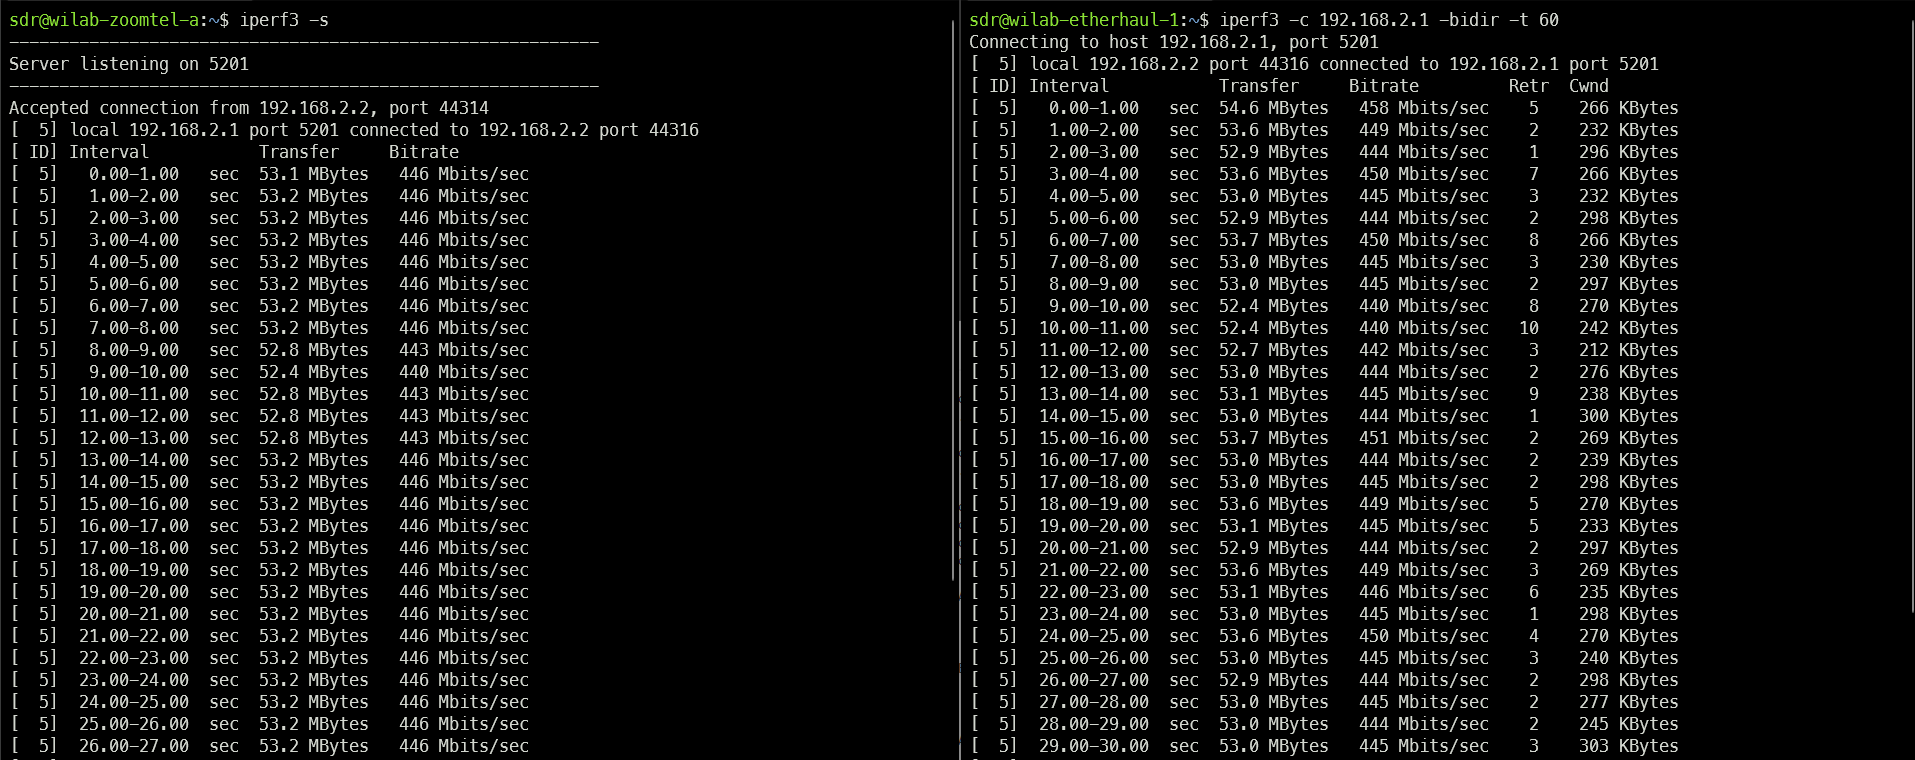
\includegraphics[width=\textwidth,keepaspectratio]{Images/Chpt3/ThroughputTest.png}
    \caption{The console output of an \textit{iperf3} test used to find the throughput for part of the ZoomTel EMANE testbed.}
    \label{iperf_test}
\end{figure}
The ZoomTel hardware testbed also used the \textit{iperf3} utility for testing.
The following command was used for running a test on the client:
\begin{minted}[fontsize=\small, breaklines]{Bash}
    iperf3 -c <server ip address> -bidir -t 60
\end{minted}
This command sets the destination of the server (the node being transmitted to) with the ``-c'' flag.
The ``-bidir'' flag indicates the test should be run in bidirectional mode so that both the throughput of the uplink and downlink can be measured.
The final flag ``-t 60'' indicates that the test should run for 60 seconds. This is to ensure a stable enough average is measured since the total throughput can have slight fluctuations.\par
The OVERCOME testbed utilized several tools for recording data.
Throughput and latency tests were measured via the website \textit{speedtest.net}~\cite{speedtest}.
This tool was used by the engineers at the Internet Service Provider that installed the equipment at the users home, and the aggregate data was found by taking an average of all results.
Users that lived closer to the center of town had better results, but this was offset in the average by houses further away.
Table~\ref{chpt3_results} shows the average results from all three environments for comparison.\par

\begin{table}
\centering
\caption{Latency and throughput measurements from the Projects OVERCOME, ZoomTel, and EMANE testbeds.}
\begin{adjustbox}{width=\textwidth, center=\textwidth}
    \begin{tabular}{l|cccc}
    \multicolumn{1}{c|}{} & Throughput (Upload) & Throughput (Download) & \multicolumn{1}{l}{Total Throughput} & Latency \\ 
    \hline
    OVERCOME & 62 Mbps & 275 Mbps & 337Mbps & 6ms \\
    ZoomTel & 87 Mbps & 87 Mbps & 174Mbps & 5.5ms \\
    EMANE & 96.6 Mbps & 96.7 Mbps & 193.2Mbps & 10ms
    \end{tabular}
\end{adjustbox}
\label{chpt3_results}
\end{table}

There are several discrepancies in the data to address.
These discrepancies do not necessarily imply the EMANE model is unreliable, but it does mean that further refinement and testing should be conducted to ensure accuracy.
Without conducting this further verification, EMANE can not be used on its own for testing as the results can not be fully trusted.\par
The first point of interest is the difference in total throughput between OVERCOME and EMANE.
OVERCOME has a much higher total throughput than EMANE, but this is likely attributed to inaccurate configuration of the CPE devices abstracted in EMANE.
The OVERCOME hardware testbed used higher end LTU radios as CPE and the configuration of the LTU model in EMANE was aligned more with the inexpensive LTU units used in the ZoomTel testbed.
This is why the results from ZoomTel and EMANE are much similar.
The uneven speeds in the OVERCOME testbed were a design decision made to allow homes to have higher download speeds.
This asymmetric behavior could not be modeled in EMANE as the generic rfPipe model does not support this functionality.
The latency differences between EMANE and the hardware testbeds is possibly attributed to the packet completion rate curves for the rfPipe models.
These curves may not have been modified enough from the baseline to line up with the actual expected behavior.
Another possibility is the delay parameters not being configured properly.
The values chosen were rather conservative estimates and may have been too high to properly model the accurate behavior of the hardware wireless signal.\par
Looking at the throughput and latency of the rfPipe model is not necessarily enough to declare that rfPipe is fully accurate to a hardware model as factors such as power and noise calculations should be verified as well.
Additionally, since EMANE models are highly configurable, any given configuration would also need to be subjected to some level of scrutiny to ensure it is accurate enough for the intended use case.

\section{Chapter Summary}
This chapter outlines how EMANE was used to create digital models of two separate wireless hybrid network topologies that were designed with the intention of delivering broadband to harder to service areas.
The architectures of both testbeds were detailed and the hardware equipment being modeled was outlined.
We then explained the parameters in EMANE that were selected in order to mimic the behavior of the hardware radios. Two rfPipe models were created, one for mmWave and one for LTU.
After building an extensive enough understanding of the transport models within EMANE, a virtual pfSense router was also brought into the loop to create additional accuracies.
The chapter finishes off by showing throughput and latency measurements taken on all testbeds and comparing them.
The results are similar enough that the emulator could be used for initial testing in place of the hardware testbed, but the discrepancies show there is room for further refinement of the emulation model.
Using a more custom model besides rfPipe could also result in better results, but this new model would need to be vigorously tested to ensure its validity.    %% OVERCOME/ZoomTEL Rural Broadband test-bed

\chapter{Intelligent Router}
\label{chapter4}

    % Broadband in rural situations is limited due to reasons explained in Chapter 3
    % Utilizes the OVERCOME test-bed from Chapter 3

\section{Intelligent Method of Bandwidth Distribution}
    % A heuristic based router that intelligently allocates bandwidth to hosts
    % Based on the behavior of uploads and downloads

\section{Implementation Methodology}
    % Want to classify each host's current upload/download usage
        % Use 
    % Use this classification to create priority tiers that influence how users get more bandwidth/bandwidth taken away
        % What is the rationale behind these priorities (study on what types of behaviors use what types of bandwidth)
    % Create these modifications to move bandwidth caps up and down via pfSense limiters


\section{Why was it implemented this way?}
    % Heuristic behavior was selected over a machine learning model
        % Why?
    % Privacy concerns
        % Did not want to classify based on the traffic type and what the user was doing
        % To create a fair algorithm can not define one type of traffic as "more important"
            % Is a Zoom call more important than a Netflix stream?
            % Business vs. Pleasure BUT Zoom is not always business and Netflix is not always leisure
    % Designed to be more system agnostic (tested on a pfSense Router)

\section{Program Effectiveness}
    % Only one iteration was able to be performed
    % Not enough traffic/users on the network for meaningful data
        % At no point during any test was total network utilization above 50%, can't take bandwidth from users to give to others if there is always a pool
    % Ways to modify/fix the experiment and test environment to create a meaningful test


\section {Chapter Summary}

    %% Intelligent Router

\chapter{Dynamic Robot Swarm Networks}
\label{chapter5}

	% This is the third use-case for EMANE
		% Combinatation use-case:
			% Work with other software
			% Emulate a distributed, dynamic network
	
	% Overview of the swarm + swarm network architecture
		% Swarm of 25 robots deployed to make environmental observations
		% Example deployment to wildfire (hostile area, remote)		
		
	% Use wireless comm links to share information with each other to:
		% Maintain the network
		% Share information between robots (to make better decisions)
		% Return information back to central command
		
	% This network is a MANET (EMANE's specialty)
		% Routing is key (the links connect and disconnect rapidly)
    

\section{Extending Existing Software}

    % Introduce ARGoS
    		% A discrete-event (?) robot swarm simulator  
        % ARGoS models the behavior of robots in the network and the environment they operate in
			% How they move
			% What data they need to be transferred
				% Based on operating algorithms
        % ARGoS operates in chunks of time instead of real, continuous time like EMANE
        		% Configurable, but for the purpose here ARGoS simulates 100ms at a time
        		% Important to understand the time-scale differences
        			% Will impact integration methodologies

	% Why integrate EMANE with ARGoS?
		% Introduce more accurate communication modeling
			% ARGoS can perform basic communication modeling
				% One example of implementation is check for line of sight conditions
				% Can account for pathloss
				% No measure of channel effects
					% Pathloss, TX/RX Power level
					% Packet corruption, delay, duplication
					% Latency
					% Throughput   		
		% Can use the full implementation of B.A.T.M.A.N. or other routing/networking software
			% Instead of coding the behavior of B.A.T.M.A.N. (or other routing from scratch) and having to verify it is functionally the same, use EMANE to run actual B.A.T.M.A.N.
				% The behavior can't be different if the program is the exact same as would be used in hardware
		% Introduce machine learning to influence routing software
            % Machine learning models can run in real time in each EMANE node, and can communicate with other models and nodes through the EMANE network
            % Allows the same models to run in EMANE as would run on the physical robot


\section{Integrating the Software}

    % Two simulation/emulation programs run simultaneous on the same machines
        % ARGoS and EMANE are both configured and run separately
            % They exist as separate processes during the extent of runtime (one is not a child of the other) 

	% A third process exists (EMANE Interface Manager)
		% EMANE on its own is a collection of programs
		% Requires something to manage all of the processes
		% Python script that runs as the broker between ARGOs and EMANE proper

    % ARGoS starts by opening shared memory and populates with metadata (including process ID) during it's initialization phase
		% (FIGURE: Shared Memory Metadata)
  		% By providing PIDs, the two programs can interact with each other
	% ARGoS then goes to sleep after initialization, waiting for EMANE-Interface to find the shared memory, and do its setup
		% Since the location of the shared memory is known, one of the processes (the one that doesn't make it) can find information from the other without knowing the PID of the other
	% EMANE-Interface populates the rest of the metadata (primarily just its PID) and sets up a shared memory location for robot pose information (location data), and robot communication data (amount of data requested to be transferred)
		% (FIGURE: Shared Memory Pose)
		% (FIGURE: Shared Memory Comm)
		% ARGoS knows where to find these shared memories (ARGoS does not create them itself because originally EMANE was supposed to create all of them, this led to issues with step 1)
		% EMANE-Interface then sets up internal data structures to store robot information and communication before waking ARGoS and going to sleep
			% The two processes communicate with each other using POSIX signals, specifically SIGSTOP to put itself to sleep and SIGCONT to wake itself
				% These signals are nice because the OS will handle stoping and waking the processes, and as such the singals are caught and handled before arriving at the process
	% ARGoS takes its turn, moving robots, sensing the environment, etc. for 100ms before it updates information about the robot poses, and communication pairs
	% EMANE-Interface then takes its turn, simulating 100ms of communication, updates shared data, and starts ARGoS
		% This is done using a simple throughput test (iperf) to determine how much data can travel through the network to a give node
		% Because there is no way to measure 100ms of data transfer easily, EMANE-Interface extrapolates the amount of data sent by dividing the speed over 1 second by 10
	% This continues until ARGoS is finished with its experiment, at which point ARGoS starts a new experiment or terminates, informing EMANE-Interface of termination

	% This Figure shows the overall connection between the two software	
	% (FIGURE: EMANE-ARGOS Interface)


\section{Integration Design Decisions}

	% Several desisions during the design of the above proces had to be made
		% These decisions were made in the hopes to maximize performance, minimize latency, and ensure stability

	% Because EMANE operates in real-time as effectively a network (i.e., nothing happens on EMANE without it getting started by a process), EMANE continues running
		% This creates oddities with "simulation time" versus "real time" but 

    % Why were certain design decisions made?
        % Shared memory
            % Less latency than something like a socket
            % The amount and size of data is known enough that appropriate blocks of memory can be opened

        % Why abstract transmission -> (Don't send actual payload through EMANE)
            % Sending the actual payload would require lots of additional work (each robot in ARGoS would need to deliver its payload to its corresponding node in EMANE, and then retrieve any data waiting for it)
            % The payoff from this work was deemed not worth it as the behavior of informing each robot how much data it sent and received accomplished the same goal
            % The payload was not being sent with a lossless protocol so the behavior of if the data arrives or not is much more important (robots would not be retransmitting)

	% Issues with C vs Python programming languages (typing and shared memory)

\section{Integration Results}

	% EMANE and ARGoS are capable of working together
		% Demonstrate ARGoS moving EMANE nodes
		% Demonstrate EMANE returning data transmission values (?)
	% However, EMANE seriously slows down ARGoS
		% We expected this
		% EMANE is an emulator and runs at a minimum, real time
		% What 
		% Can we make it faster?

\section{Chapter Summary}

    %% DAC, ARGoS, Robot Swarms

\chapter{Conclusion}
\label{conclusion}
\section{Research Outcomes}
Overall, this project was able to achieve its primary goal of evaluating and understanding the EMANE tool.
Several scenarios were presented that EMANE was shown to be successful operating in.
The first use-case of rural broadband testing, showed that the basic rfPipe radio model can be configured to match the characteristics of a hardware testbed.
This scenario does carry the warning that just because the characteristics of the network were the same, not every model in EMANE is validated.
The rfPipe model is simple enough that the throughput and latency being similar is enough to use it in basic testing, but advance models mimic more complex models that must be examined.
The second use-case shows that EMANE provides an ideal environment for testing and developing networking software.
Care must be taken when modeling test traffic, but EMANE provides many avenues for creating and using test data.
The third use case shows that EMANE is able to work with other tools to create a more complete system, with the timescale differences identified as the major obstacle to be considered.

\section{Future Work}
    % Create more accurate and refined models for EMANE that can then be pluggable into testbeds
        % Once these models are created, more advance wireless emulation can be done with similar ease thanks to the plug and play nature of EMANE
        % These models would will need to be vigorously tested to ensure the validity of the results
    % Further testing of the intelligent router program in more appropriate conditions
    % Further integrations between ARGoS and EMANE to expand functionality and optimize time consumed
While each stage of this thesis had successes, there are still several pieces of work that remain uncompleted. The following list outlines this future work:
\begin{itemize}
    \item Conducting extensive validation of the models included within EMANE. EMANE is not as widely used as many other network testing tools, and as such has been studied less for its validity. If more advanced models are to be used in EMANE, it should be ensured they are accurate enough for the advanced use cases.
    \item Creating additional wireless models for EMANE. By default, EMANE only has radio models accessible, with one being the generic model used in this thesis and another being used for testing of EMANE itself. If EMANE is to be more widely used, it needs to be able to model more modern waveforms and technologies.
    \item Additional testing and development of the intelligent router software. Due to the issues described in Chapter~\ref{chapter2} only one initial test was conducted with non-ideal conditions.
    \item Further integration and optimizations between EMANE and ARGoS. Finding ways to reduce the time EMANE adds onto the total simulation, while also adding functionality to allow for modeling of more communication factors like latency or advanced routing techniques would allow the integration to be even more widely used.
\end{itemize}  %% Closing thoughts/future work

%%%%%%%%%%%%%%%%%%%%%%%%%%%%%%%%%% THE END %%%%%%%%%%%%%%%%%%%%%%%%%%%%%%%%%
%SEE HERE for BIBTEX styles: http://www.cs.stir.ac.uk/~kjt/software/latex/showbst.html
\bibliographystyle{IEEEtran}
\bibliography{references}

\appendix
\chapter{Installation of EMANE}   %% Installation of EMANE

\end{document}
